
%  PLEASE DO NOT REMOVE OR CHANGE THIS BLOCK
%  ===========================================================
%
%  A LaTeX Template for Typesetting Theses in Persian
%  By: Hamid Zarrabi-Zadeh
%  Source: https://github.com/zarrabi/thesis-template
%
%  License: Creative Commons Attribution 4.0
%  https://creativecommons.org/licenses/by/4.0/
%
%  Contributors: Ehsan Emamjomeh-Zadeh and Omid Gheibi
%  See the full list of contributors at GitHub.
%
%  ===========================================================


\documentclass[oneside,a4paper,12pt]{book}


% -------------------------------------------------------
%  Common Styles and Formattings
% -------------------------------------------------------

\usepackage{amssymb,amsmath}
\usepackage[colorlinks,linkcolor=blue,citecolor=blue]{hyperref}
\usepackage[usenames,dvipsnames]{pstricks}
\usepackage{graphicx,subfigure,wrapfig}
\usepackage{geometry}

%\usepackage{listings}
%\definecolor{dkgreen}{rgb}{0,0.6,0}
%\definecolor{gray}{rgb}{0.5,0.5,0.5}
%\definecolor{mauve}{rgb}{0.58,0,0.82}
%
%\lstset{frame=tb,
%	language=Python,
%	aboveskip=3mm,
%	belowskip=3mm,
%	showstringspaces=false,
%	columns=flexible,
%	basicstyle={\small\ttfamily},
%	numbers=none,
%	numberstyle=\tiny\color{gray},
%	keywordstyle=\color{blue},
%	commentstyle=\color{dkgreen},
%	stringstyle=\color{mauve},
%	breaklines=true,
%	breakatwhitespace=true,
%	tabsize=1
%}

\usepackage[mathscr]{euscript}
\usepackage{multicol}
\usepackage{multirow}
\usepackage[figureposition=bottom,tableposition=top,font={small,bf},labelfont=bf]{caption}

\usepackage{tablefootnote}
%\usepackage[hang]{footmisc}
%\setlength{\footnotemargin}{2mm}
\usepackage{algorithmicx,algorithm}

\usepackage[most]{tcolorbox}
\tcbuselibrary{listingsutf8}

\usepackage[localise=on,extrafootnotefeatures]{xepersian}
\usepackage[noend]{algpseudocode}


%------------------------ Algorithm ------------------------------------

\newenvironment{الگوریتم}[1]
	{\bigskip\bigskip\begin{algorithm}\caption{#1} \label{الگوریتم: #1}\vspace{0.5em}\begin{algorithmic}[1]}
	{\end{algorithmic}\vspace{0.5em}\end{algorithm}\bigskip}
	

\renewcommand{\algorithmicfor}{{به ازای}}
\renewcommand{\algorithmicwhile}{{تا وقتی}}
\renewcommand{\algorithmicdo}{\hspace{-.2em}:}
\renewcommand{\algorithmicif}{{اگر}}
\renewcommand{\algorithmicthen}{\hspace{-.2em}:}
\renewcommand{\algorithmicelse}{{در غیر این صورت:}}
%\renewcommand{\algorithmicelsif}{{در غیر این صورت اگر: }}
\renewcommand{\algorithmicreturn}{{برگردان}}
\renewcommand{\algorithmiccomment}[1]{$\triangleleft$ \emph{#1}}
\renewcommand{\algorithmicrequire}{\textbf{ورودی:}}
\renewcommand{\algorithmicensure}{\textbf{خروجی:}}

\newcommand{\اگر}{\If}
\newcommand{\وگرنه}{\Else}
\newcommand{\وگر}{\ElsIf}
\newcommand{\پایان‌اگر}{\EndIf}
\newcommand{\به‌ازای}{\For}
\newcommand{\پایان‌به‌ازای}{\EndFor}
\newcommand{\تاوقتی}{\While}
\newcommand{\پایان‌تاوقتی}{\EndWhile}
\newcommand{\دستور}{\State}
\newcommand{\دستورک}{\Statex}
\newcommand{\توضیحات}{\Comment}
\newcommand{\برگردان}{\Return}
\renewcommand{\ورودی}{\Require}
\newcommand{\خروجی}{\Ensure}



% -------------------- Page Layout --------------------


%\newgeometry{top=3cm,right=3cm,left=2.5cm,bottom=3cm,footskip=1.25cm}
\newgeometry{margin=1in,bottom=1.1in,footskip=.4in}

\renewcommand{\baselinestretch}{1.4}
\linespread{1.6}
\setlength{\parskip}{0.45em}

%\fancyhf{}
%\rhead{\leftmark}
%\lhead{\thepage}

\sloppy


% -------------------- Default Font --------------------

\settextfont[
	Scale=1.09,
	Extension=.ttf,
	Path=styles/fonts/,
	BoldFont=XB NiloofarBd,
	ItalicFont=XB NiloofarIt,
	BoldItalicFont=XB NiloofarBdIt
]{XB Niloofar}

\setdigitfont[
	Scale=1.09,
	Extension=.ttf,
	Path=styles/fonts/,
	BoldFont=XB NiloofarBd,
	ItalicFont=XB NiloofarIt,
	BoldItalicFont=XB NiloofarBdIt
]{XB Niloofar}


% -------------------- Sharif Font --------------------

\newcommand{\shariffont}{
	\settextfont[
		Scale=1.4,
		Extension=.ttf,
		Path=styles/fonts/,
		BoldFont=Sharif1.3-SemiBold,
	]{Sharif1.3-Regular}

	\setdigitfont[
		Scale=1.4,
		Extension=.ttf,
		Path=styles/fonts/,
		BoldFont=Sharif1.3-SemiBold,
	]{Sharif1.3-Regular}
}

% -------------------- Styles --------------------


\SepMark{-}
\renewcommand{\labelitemi}{$\small\bullet$}



% -------------------- Environments --------------------


\newtheorem{قضیه}{قضیه‌ی}[chapter]
\newtheorem{لم}[قضیه]{لم}
\newtheorem{ادعا}[قضیه]{ادعای}
\newtheorem{مشاهده}[قضیه]{مشاهده‌ی}
\newtheorem{نتیجه}[قضیه]{نتیجه‌ی}
\newtheorem{مسئله}{مسئله‌ی}[chapter]
\newtheorem{تعریف}{تعریف}[chapter]
\newtheorem{مثال}{مثال}[chapter]


\newenvironment{اثبات}
{\begin{trivlist}\item[\hskip\labelsep{\em اثبات.}]}
		{\leavevmode\unskip\nobreak\quad\hspace*{\fill}{\ensuremath{{\square}}}\end{trivlist}}

\newenvironment{alg}[2]
{\begin{latin}\settextfont[Scale=1.0]{Times New Roman}
		\begin{algorithm}[t]\caption{#1}\label{algo:#2}\vspace{0.2em}\begin{algorithmic}[1]}
				{\end{algorithmic}\vspace{0.2em}\end{algorithm}\end{latin}}


% -------------------- Titles --------------------


\renewcommand{\listfigurename}{فهرست شکل‌ها}
\renewcommand{\listtablename}{فهرست جدول‌ها}
\renewcommand{\bibname}{\rl{{مراجع}\hfill}}


% -------------------- Commands --------------------


\newcommand{\IN}{\ensuremath{\mathbb{N}}}
\newcommand{\IZ}{\ensuremath{\mathbb{Z}}}
\newcommand{\IQ}{\ensuremath{\mathbb{Q}}}
\newcommand{\IR}{\ensuremath{\mathbb{R}}}
\newcommand{\IC}{\ensuremath{\mathbb{C}}}

\newcommand{\set}[1]{\left\{ #1 \right\}}
\newcommand{\seq}[1]{\left< #1 \right>}
\newcommand{\ceil}[1]{\left\lceil{#1}\right\rceil}
\newcommand{\floor}[1]{\left\lfloor{#1}\right\rfloor}
\newcommand{\card}[1]{\left|{#1}\right|}
\newcommand{\setcomp}[1]{\overline{#1}}
\newcommand{\provided}{\,:\,}
\newcommand{\divs}{\mid}
\newcommand{\ndivs}{\nmid}
\newcommand{\iequiv}[1]{\,\overset{#1}{\equiv}\,}
\newcommand{\imod}[1]{\allowbreak\mkern5mu(#1\,\,\text{پیمانه‌ی})}

\newcommand{\poly}{\mathop{\mathrm{poly}}}
\newcommand{\polylog}{\mathop{\mathrm{polylog}}}
\newcommand{\eps}{\varepsilon}

\newcommand{\lee}{\leqslant}
\newcommand{\gee}{\geqslant}
\renewcommand{\leq}{\lee}
\renewcommand{\le}{\lee}
\renewcommand{\geq}{\gee}
\renewcommand{\ge}{\gee}

\newcommand{\مهم}[1]{\textbf{#1}}
\renewcommand{\برچسب}{\label}

\newcommand{\REM}[1]{}
\renewcommand{\حذف}{\REM}
\newcommand{\لر}{\lr}
\newcommand{\کد}[1]{\lr{\tt #1}}
\newcommand{\پاورقی}[1]{\footnote{\lr{#1}}}



% -------------------- Dictionary --------------------


\newcommand{\dicalphabet}[1]{
	\begin{minipage}{\columnwidth}
		\centerline{\noindent\textbf{\large #1 }}
		\vspace{.5em}
	\end{minipage}
	\nopagebreak[4]
}

\newcommand{\dic}[2]{\noindent  #2 \dotfill  \lr{#1} \\ }


% ------------------------------ Images and Figures --------------------------

\graphicspath{{figs/}}
\setlength{\intextsep}{0pt}  % for float boxes
\renewcommand{\psscalebox}[1]{}  % for LaTeX Draw

\newcommand{\floatbox}[2]
{\begin{wrapfigure}{l}{#1}
		\centering #2 \end{wrapfigure}}

\newcommand{\centerfig}[2]
{\centering\scalebox{#2}{\input{figs/#1}}}

\newcommand{\fig}[3]
{\floatbox{#3}{\centerfig{#1}{#2}}}

\newcommand{\centerimg}[2]
{\vspace{1em}\begin{center}\includegraphics[width=#2]{figs/#1}\end{center}\vspace{-1.5em}}

\NewDocumentCommand{\img}{m m o}
{\begin{wrapfigure}{l}{\IfValueTF{#3}{#3}{#2}}
		\centering\includegraphics[width=#2]{figs/#1}\end{wrapfigure}}




% -------------------------------------------------------
%  Custom Definitions
% -------------------------------------------------------


\newcommand{\OPT}{\ensuremath{\mathop{\mathrm{OPT}}}}
\newcommand{\APX}{\ensuremath{\mathop{\mathrm{APX}}}}
\newcommand{\ALG}{\ensuremath{\mathop{\mathrm{ALG}}}}



\begin{document}


% -------------------- Font Settings --------------------

\shariffont  % برای استفاده از فونت شریف این خط را فعال کنید


% -------------------- Front Pages --------------------


% -------------------------------------------------------
%  Thesis Information
% -------------------------------------------------------

\newcommand{\ThesisType}
{پایان‌نامه}  % پایان‌نامه / رساله
\newcommand{\ThesisDegree}
{کارشناسی}  % کارشناسی / کارشناسی ارشد / دکتری
\newcommand{\ThesisMajor}
{علوم کامپیوتر}  % نام رشته / گرایش
\newcommand{\ThesisTitle}
{ترمیم تصاویر بر پایه معماری Transformers و بررسی روش های مرسوم}  % عنوان پایان‌نامه / رساله
\newcommand{\ThesisAuthor}
{نوید مافی رنجی}  % نام نویسنده
\newcommand{\ThesisSupervisor}
{دکتر کیمیا پیوندی}  % نام استاد راهنما
\newcommand{\ThesisAdvisor}
{دکتر کیمیا پیوندی}
\newcommand{\ThesisExaminer}
{دکتر علیرضا نعیمی}
\newcommand{\ThesisDate}
{زمستان ۱۴۰۳}
\newcommand{\ThesisDepartment}
{دانشکده ریاضی، آمار و علوم کامپیوتر}
\newcommand{\ThesisUniversity}
{دانشگاه سمنان}

% -------------------------------------------------------
%  English Information
% -------------------------------------------------------

\newcommand{\EnglishThesisDegree}{B.Sc.}

\newcommand{\EnglishThesisTitle}{Towards Synthesizing Large-Scale Low-Light Imaging Datasets via Training Deep Learning Models}

\newcommand{\EnglishThesisAuthor}{Navid Mafi Ranji}

\newcommand{\EnglishThesisSupervisor}{Dr. Kimia Peivandi}

\newcommand{\EnglishThesisDate}{Winter 2024}

\newcommand{\EnglishThesisDepartment}{Department of Computer Science}

\newcommand{\EnglishThesisUniversity}{Semnan University}

\pagestyle{empty}

% -------------------------------------------------------
%  Title Page
% -------------------------------------------------------


% راهنمایی: اطلاعات پایان‌نامه را در فایل front/info.tex ویرایش کنید.

\begin{center}

    
\includegraphics[scale=0.5]{front/template/images/logo}

    \vspace{-0.2cm}
    \ThesisUniversity \\[-0.3em]
    \ThesisDepartment

    \begin{large}
        \vspace{0.5cm}

        \ThesisType \ \ThesisDegree \\[-0.3em]
        \ThesisMajor

    \end{large}

    \vspace{2cm}

    {\LARGE\textbf{\ThesisTitle}}

    \vspace{2.5cm}

    {نگارش}\\[.5em]
    {\large\textbf{\ThesisAuthor}}

    \vspace{0.7cm}

    {استاد راهنما}\\[.5em]
    {\large\textbf{\ThesisSupervisor}}

    \vspace{1.3cm}

    \ThesisDate

\end{center}



% info: برای درج هر یک از صفحات زیر، خط مربوطه را فعال کنید

%
% -------------------------------------------------------
%  Besmellah Page
% -------------------------------------------------------

\begin{center}


\includegraphics[width=0.45\textwidth]{front/template/images/besmellah}

\end{center}
  % صفحه بسم الله
%
% -------------------------------------------------------
%  Signatures Page
% -------------------------------------------------------

\begin{large}
\setlength{\parindent}{0pt}
\begin{center}

%{\large\bf تصویب‌نامه}\\
\vspace{1em}

{\normalsize\bf به نام خدا}

{\normalsize
\ThesisUniversity\\[-0.1cm]
\ThesisDepartment}

\vspace{2.5em}
\textbf{\large\ThesisType \ \ThesisDegree}

\vspace{0.5em}
این \ThesisType\ به عنوان تحقق بخشی از شرایط دریافت درجه \ThesisDegree\ است.
\end{center}

\vspace{1.5em}

{\large \textbf{عنوان}: \ThesisTitle}

\vspace{.3em}

{\large \textbf{نگارش}: \ThesisAuthor}

\vspace{1cm}

\textbf{کمیته ممتحنین}

\vspace{1em}
\begin{tabular}{p{7cm}r}
استاد راهنما: \ThesisSupervisor & امضاء: \\[1.5em]
استاد مشاور: \ThesisAdvisor & امضاء: \\[1.5em]
استاد مدعو: \ThesisExaminer & امضاء: \\[2em]
& تاریخ:
\end{tabular}

\end{large}

  % صفحه تصویب‌نامه
%
% -------------------------------------------------------
%  Declaration Page
% -------------------------------------------------------

{\parindent0pt

\begin{center}
	{\large\bf اظهارنامه}

	{\small(اصالت متن و محتوای \ThesisType{} \ThesisDegree)}
\end{center}
\vspace{-6em}

\includegraphics[scale=0.18]{front/template/images/logo}

\vspace{1em}

\textbf{عنوان ‌\ThesisType}: \ThesisTitle

\vspace{.1em}
\begin{multicols}{2}
	{\مهم{استاد راهنما}: \ThesisSupervisor}

	{\مهم{استاد مشاور}: \ThesisAdvisor}
\end{multicols}

\vspace{0.2em}
\کوچک
این‌جانب {\ThesisAuthor} اظهار می‌دارم:
\شروع{شمارش}
\فقره متن و نتایج علمی ارائه شده در این \ThesisType{} اصیل بوده و زیرنظر استادان نام‌برده ‌شده در بالا تهیه شده است.
\فقره متن \ThesisType{} به این صورت در هیچ جای دیگری منتشر نشده است.
\فقره متن و نتایج مندرج در این \ThesisType، حاصل تحقیقات این‌جانب به عنوان دانشجوی \ThesisDegree{} دانشگاه صنعتی شریف است.
\فقره کلیه مطالبی که از منابع دیگر در این \ThesisType{} مورد استفاده قرار گرفته، با ذکر مرجع مشخص شده است.
\پایان{شمارش}

\begin{multicols}{2}
	\ \\
	\ \\
	\ \\

	نگارنده: \ThesisAuthor\\
	تاریخ: \\
	امضاء: \\
\end{multicols}

نتایج تحقیقات مندرج در این \ThesisType{} و دستاوردهای مادی و معنوی ناشی از آن (شامل فرمول‌ها، توابع کتابخانه‌ای، نرم‌افزارها، سخت‌افزارها و مواردی که قابلیت ثبت اختراع دارد) متعلق به دانشگاه صنعتی شریف است. هیچ شخصیت حقیقی یا حقوقی بدون کسب اجازه از دانشگاه صنعتی شریف حق فروش و ادعای مالکیت مادی یا معنوی بر آن یا ثبت اختراع از آن را ندارد. همچنین، کلیه حقوق مربوط به چاپ، تکثیر، نسخه‌برداری، ترجمه، اقتباس و نظائر آن در محیط‌های مختلف اعم از الکترونیکی، مجازی یا فیزیکی برای دانشگاه صنعتی شریف محفوظ است. نقل مطلب با ذکر ماخذ بلامانع است.


\begin{multicols}{2}
	استاد راهنما: \ThesisSupervisor \\
	تاریخ: \\
	امضاء: \\

	نگارنده: \ThesisAuthor\\
	تاریخ: \\
	امضاء: \\
\end{multicols}
}

  % صفحه اظهارنامه

\pagestyle{plain}
\pagenumbering{tartibi}


% -------------------------------------------------------
%  Acknowledgments
% -------------------------------------------------------


\begin{center}
    \مهم{سپاس}
\end{center}

از استادان بزرگوارم که با کمک‌ها و راهنمایی‌های بی‌دریغشان، مرا
در به سرانجام رساندن این پایان‌نامه یاری داده‌اند، تشکر و قدردانی می‌کنم.
همچنین از همکاران عزیزی که با راهنمایی‌های خود در بهبود نگارش این نوشتار
سهیم بوده‌اند، صمیمانه سپاسگزارم.
%
%زیرساخت های بسیار غنی دانشگاه سمنان و دسترسی بسیار آسان به امکاناتی ابتدایی همچون ایمیل دانشجویی، کار را برای ما بسیار بهبود بخشید. (به شکل \ref{fig:screenshot001} توجه شود) 
%\\
%\\
%
%
%\begin{figure}[h]
%	\centering
%	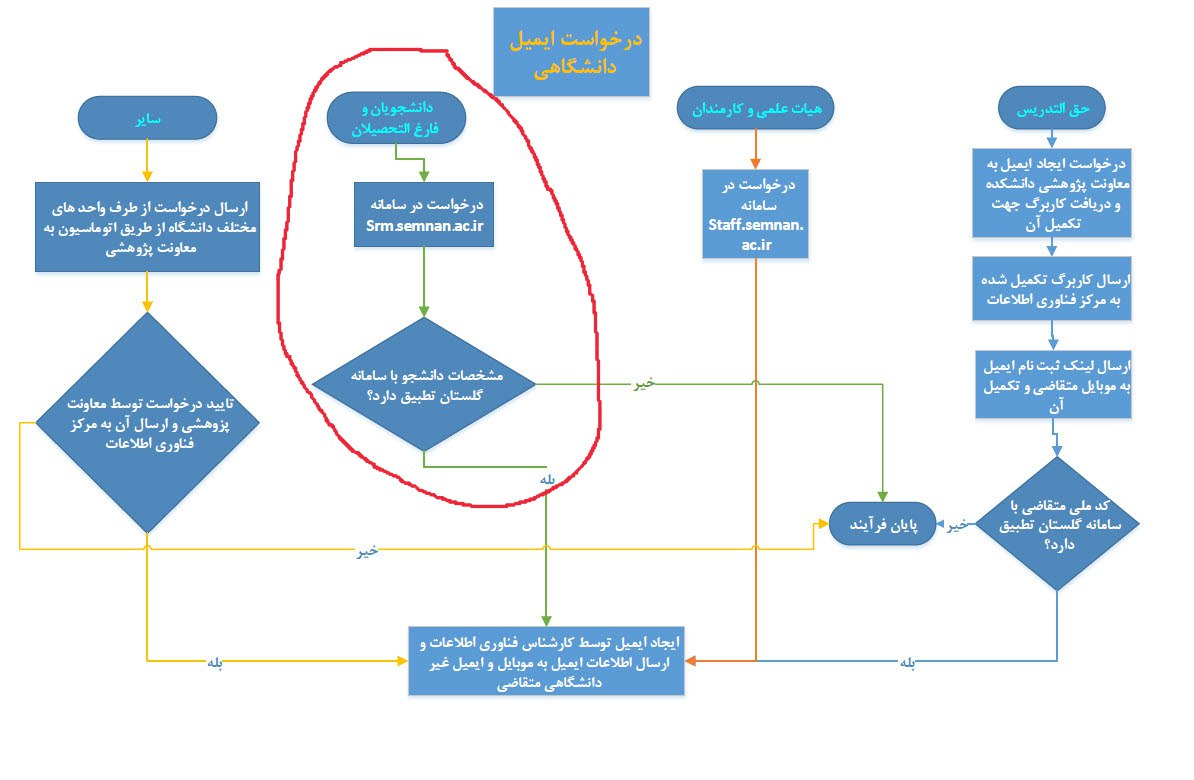
\includegraphics[width=1\linewidth]{screenshot002}
%	
\includegraphics[width=1\linewidth]{screenshot001}
%	\caption{دسترسی بسیار آسان به منابعی مانند ایمیل دانشجویی}
%	\label{fig:screenshot001}
%\end{figure}
%

  % صفحه سپاس

% -------------------------------------------------------
%  Abstract
% -------------------------------------------------------


\شروع{وسط‌چین}
\مهم{چکیده}
\پایان{وسط‌چین}
\بدون‌تورفتگی
ترمیم تصاویر، به‌عنوان یکی از چالش‌های اصلی در پردازش تصویر، با هدف بازسازی قسمت‌های از‌دست‌رفته یا آسیب‌دیده‌ی تصاویر بدون تخریب ساختار بصری و مفهومی انجام می‌شود. روش‌های مرسوم ترمیم، شامل تکنیک‌های الگوریتمی و یادگیری‌محور، اغلب در شرایط پیچیده مانند بازیابی جزئیات دقیق یا بازسازی بافت‌های پیچیده محدودیت‌هایی دارند. در این پژوهش، یک مدل نوین مبتنی بر معماری Transformers پیشنهاد شده است که با بهره‌گیری از قدرت مکانیزم توجه، عملکرد قابل‌توجهی در بازیابی ساختار و جزئیات ارائه می‌دهد.


در این مطالعه، پس از مرور جامع بر روش‌های پیشین و ارزیابی محدودیت‌های آن‌ها، اصلاحاتی در معماری Transformer استاندارد اعمال شده و کارایی آن با استفاده از معیارهای استاندارد مانند SSIM و PSNR سنجیده شده است. همچنین، آزمایش‌های جانبی با استفاده از LSTM‌ ها بر روی داده‌های غیرزمانی انجام شده که اگرچه به نتیجه مطلوب نرسیدند، اما بینش‌های ارزشمندی در خصوص ویژگی‌های این داده‌ها ارائه کردند. 


\پرش‌بلند
\بدون‌تورفتگی \مهم{کلیدواژه‌ها}: 
ترمیم تصویر، ترنسفورمر، مکانیزم توجه، شبکه های عصبی
\صفحه‌جدید



% -------------------- Table of Contents --------------------

\tableofcontents \newpage
\listoftables \newpage
\listoffigures \newpage


% -------------------- Chapters --------------------

\pagenumbering{arabic}

%\chapter{مقدمه}
\section{تعریف مسئله}

ترمیم (تکمیل) تصاویر 
\LTRfootnote{Image Inpainting (Completion)}
یکی از شاخه‌های اساسی در حوزه پردازش تصویر است که با هدف بازسازی بخش‌های آسیب‌دیده یا حذف‌شده‌ی تصاویر به گونه‌ای انجام می‌شود که کیفیت بصری و اطلاعات معنایی تصویر حفظ گردد. این مسئله کاربردهای گسترده‌ای در زمینه‌هایی مانند ویرایش تصاویر 
\cite{joSCFEGANFaceEditing2019}
، بازیابی داده‌های تاریخی %
\cite{wanBringingOldPhotos2020, wanOldPhotoRestoration2020}%
، و کاربردهای پزشکی، صنعتی و امنیتی دارد. با این حال، به دلیل پیچیدگی ویژگی‌های بصری تصاویر، مانند الگوهای متقارن، جزئیات دقیق، و بافت‌های پیچیده، ترمیم دقیق و بدون خطا همچنان چالشی بزرگ باقی مانده است.

یکی از مشکلات اصلی در ترمیم تصاویر، حفظ وابستگی‌های طولانی‌مدت در سرتاسر تصویر است. در روش‌های معمولی مانند شبکه عصبی کانولوشنی (CNN)
\cite{laubeImageInpaintingHighResolution2018}%
، که به طور عمده بر ویژگی‌های محلی تمرکز دارند، این وابستگی‌ها به خوبی مدیریت نمی‌شوند. به این معنا که در مواقعی که نواحی بزرگی از تصویر نیاز به ترمیم دارند یا لبه‌های پیچیده‌ای باید بازسازی شوند، مدل‌های CNN قادر به درک کامل و منطقی از بافت کلی تصویر نبوده و ممکن است در تولید نواحی ترمیم‌شده دچار مشکلاتی مانند عدم هماهنگی با محیط اطراف شوند. این مشکل به‌ویژه در ترمیم نواحی بزرگ یا پیچیده‌تر از تصویر که نیاز به درک زمینه و روابط بین نواحی مختلف دارند، خود را نشان می‌دهد. به همین دلیل، استفاده از معماری‌های ترنسفورمر (Transformer)
\cite{vaswaniAttentionAllYou2023}
که از مکانیزم توجه
\LTRfootnote{Attention Mechanism}
\cite{bahdanauNeuralMachineTranslation2016}
 برای شناسایی وابستگی‌ها در سطح سراسری بهره می‌برد، می‌تواند این مشکل را به طور مؤثری حل کند. ترنسفورمر ها  که به دلیل مکانیزم توجه خود عملکرد موفقی در زمینه‌های مختلف یادگیری عمیق داشته اند، می توانند با توانایی پردازش وابستگی‌های بلندمدت، قادرند اطلاعات مورد نیاز از سرتاسر تصویر را جمع‌آوری کرده و نواحی ترمیم‌شده را به شکلی هم‌راستا و منطقی با بقیه تصویر بازسازی کنند.

\section{اهمیت موضوع}
اهمیت مسئله ترمیم تصاویر از آنجا ناشی می‌شود که این فرایند به‌طور مستقیم با کیفیت تجزیه و تحلیل و تفسیر داده‌های بصری در بسیاری از زمینه‌ها مرتبط است. در کاربردهای پزشکی، مانند بازسازی تصاویر پزشکی از سی‌تی‌اسکن‌ها یا MRI‌ ها، ترمیم تصاویر می‌تواند به تشخیص دقیق‌تر و سریع‌تر بیماری‌ها کمک کند. همچنین، در زمینه‌های امنیتی و نظارتی، بازسازی صحیح و دقیق تصاویر از محیط‌های آسیب‌دیده می‌تواند اطلاعات حیاتی برای تجزیه و تحلیل وقایع فراهم آورد. در دنیای دیجیتال امروزی، ترمیم تصاویر به‌عنوان یکی از ابزارهای اساسی در ویرایش گرافیکی و بازسازی آثار هنری تاریخی شناخته می‌شود.


\section{ادبیات موضوع}
ترمیم تصاویر یکی از مهم‌ترین چالش‌ها در حوزه پردازش تصویر است که از دیرباز مورد توجه محققین قرار گرفته است. این فرایند به‌ویژه در مواقعی که بخش‌هایی از تصویر به دلایل مختلف مانند خرابی، آسیب‌دیدگی، یا حذف عمدی از دست رفته‌اند، اهمیت ویژه‌ای پیدا می‌کند. در ابتدا، روش‌های ترمیم مبتنی بر الگوریتم‌های سنتی 

با پیشرفت تکنولوژی و ظهور شبکه‌های عصبی عمیق، به‌ویژه شبکه‌های عصبی کانولوشنی (CNN) و \rl{U-Net}، روش‌های یادگیری عمیق به ابزاری کارآمد برای ترمیم تصاویر تبدیل شدند. این مدل‌ها توانستند قابلیت‌های بالایی در بازسازی جزئیات و ساختارهای پیچیده تصاویر نشان دهند. در ادامه، روش‌هایی مانند Autoencoders (AEs) نیز به‌منظور تقویت قابلیت‌های بازسازی پیشنهاد شدند. با این حال، علی‌رغم موفقیت‌های چشمگیر این رویکردها، همچنان در بازسازی دقیق و بی‌عیب تصاویر پیچیده و بافت‌های ظریف چالش‌هایی وجود دارد.

تحقیقاتی که به استفاده از معماری‌های پیشرفته‌تری مانند مکانیزم توجه پرداخته‌اند، این امکان را فراهم کرده‌اند که مدل‌ها به درک بهتر روابط بلندمدت و جزئیات ظریف‌تر در داده‌ها دست یابند. به‌ویژه، معماری ترنسفورمر به دلیل ساختار قابل‌موازی‌سازی و مکانیزم توجه‌محور، انقلابی در پردازش تصویر و زبان ایجاد کرده است. استفاده از این معماری‌ها در ترمیم تصاویر می‌تواند گامی مؤثر در جهت بهبود کیفیت و دقت ترمیم تصاویر با پیچیدگی‌های بیشتر باشد.


\section{اهداف پژوهش}

در این تحقیق، هدف اصلی بررسی کاربرد معماری‌های ترنسفورمر در حوزه ترمیم تصاویر است. یکی از چالش‌های بزرگ در ترمیم تصاویر، توانایی مدل‌ها در حفظ همبستگی‌های بلندمدت و منطقی در سراسر تصویر است. در حالی که شبکه‌های CNN معمولاً برای استخراج ویژگی‌های محلی مناسب هستند، مشکل آنها در مدیریت وابستگی‌های بلندبرد و ایجاد همبستگی‌های طبیعی در نواحی بزرگ تصویر مشهود است.

یکی دیگر از اهداف تحقیقاتی، بررسی چگونگی استفاده از مدل‌های ترنسفورمر برای بهبود کارایی و سرعت فرآیند ترمیم است. در حالی که مدل‌های RNN و LSTM در گذشته برای پردازش داده‌های ترتیبی استفاده می‌شدند، این مدل‌ها در پردازش داده‌های غیر ترتیبی مانند تصاویر با مشکل مواجه هستند. به طور خاص، این مدل‌ها به دلیل پردازش ترتیبی و وابستگی به مراحل قبلی، زمان‌بر و کند هستند. در مقابل، ترنسفورمر ها با پردازش موازی داده‌ها، به مدل‌ها این امکان را می‌دهد که به طور کارآمدتری پردازش کنند و زمان پردازش را برای تصاویر با ابعاد بزرگ کاهش دهند. این تحقیق به دنبال ارزیابی این مزیت برای ترمیم تصاویر است.

یکی از اهداف فرعی تحقیق، تحلیل و مقایسه عملکرد ترنسفورمر با سایر روش‌های رایج در ترمیم تصاویر مانند GAN و U-Net است. در حالی که مدل‌های GAN در تولید تصاویر از کیفیت بالایی برخوردارند، از نظر پایداری در فرآیند آموزش و توانایی برای ترمیم نواحی بزرگ و پیچیده، همچنان با مشکلاتی مواجه هستند. همچنین، U-Net که یکی از مدل‌های موفق در ترمیم تصویر است، بیشتر به ویژگی‌های محلی توجه دارد و گاهی در ترمیم نواحی بزرگ‌تر یا پیچیده‌تر دچار مشکلاتی می‌شود. تحقیق حاضر به دنبال نشان دادن مزایای ترنسفورمر در رفع این مشکلات و ارائه نتایج بهبود یافته است.

در نهایت، این تحقیق با ارائه رویکردهایی برای ترکیب معماری‌های مختلف، مانند LSTM و ترنسفورمر در ترمیم تصاویر، به دنبال شناسایی الگوهای جدیدی برای بهبود عملکرد مدل‌ها است. یکی از جنبه‌های مهم این تحقیق، ارزیابی نتایج با استفاده از معیارهای معتبر همچون SSIM و PSNR است تا اثبات کند که تغییرات معماری پیشنهادی در نهایت به بهبود کیفیت ترمیم تصاویر می‌انجامد. همچنین، آزمایش‌های ناموفق قبلی با LSTM در ترمیم غیرزمانی به طور مفصل بررسی خواهد شد تا بینش‌های جدیدی از آن‌ها استخراج گردد و به توسعه مدل‌های آینده کمک کند.


\section{ساختار پایان‌نامه}

این پایان‌نامه در شش فصل تنظیم شده است که هرکدام به جنبه‌های مختلف تحقیق و تحلیل مدل‌های ترمیم تصویر می‌پردازد. در ادامه، در فصل دوم، مفاهیم کلیدی مرتبط با ترمیم تصویر و معماری‌های مختلف مانند CNN ها، RNN ها،‌ مدل های GAN و ترنسفورمر شرح داده می‌شود. در فصل سوم، مروری بر مطالعات، روش‌ها و مجموعه داده‌ها
\LTRfootnote{Datasets}
ی ترمیم تصویر، تاریخچه روش‌های ترمیم تصویر، به ویژه مدل‌های مبتنی بر یادگیری عمیق مانند GAN و U-Net بررسی می‌شود. در این فصل همچنین به تحلیل مزایا و معایب این روش‌ها پرداخته خواهد شد. فصل چهارم، معماری‌های شبکه عصبی و پیشرفت‌ها در معماری‌های ترنسفورمر، به توضیح تاریخچه RNNها و LSTMها، مکانیزم‌های توجه و Transformers در پردازش زبان طبیعی و بینایی ماشین پرداخته و کاربرد این مدل‌ها را در ترمیم تصویر مورد بررسی قرار می‌دهد. فصل پنجم، روش‌های پیشنهادی و آزمایش‌ها، به ارائه روش‌های جدید و تغییرات در معماری های ترمیم تصاویر می پردازد. در نهایت، در فصل ششم نتایج را بررسی و جمع‌بندی می‌کنیم و پیشنهاداتی برای بهبود روش‌های آتی ارائه می‌دهیم.
%
\chapter{مفاهیم اولیه}

در این فصل،‌ ابتدا مسئله ترمیم تصویر را بطور مفصل تشریح و تعریف کرده و معماری‌های پایه را بررسی می‌کنیم. سپس به بررسی مجموعه‌داده‌های استفاده شده در یادگیری این روش ها می‌پردازیم.

\section{مسئله ترمیم تصویر}


ترمیم تصویر به معنای بازسازی نواحی گمشده یا خراب در یک تصویر است. این نواحی ممکن است به دلایل مختلفی مانند آسیب فیزیکی به تصویر، حذف بخش‌هایی از تصویر یا نقص داده‌ها در حین پردازش رخ دهند. مسئله ترمیم تصویر را می‌توان به‌طور ریاضی به صورت زیر بیان کرد:

فرض کنید که یک تصویر \(I\) از ابعاد \(H \times W\) داریم که بخشی از آن خراب یا گمشده است. تصویر خراب‌شده را می‌توان به صورت \(I_{\text{observed}}\) نمایش داد که به‌طور جزئی از \(I\) در نواحی مشخص شده توسط یک ماتریس ماسک \(M\) به‌دست آمده است. به این صورت که:

\[
I_{\text{observed}} = M \odot I
\]

در این رابطه، \(\odot\) نشان‌دهنده ضرب عنصر به عنصر است و \(M\) یک ماتریس باینری است که در آن مقادیر 1 به نواحی دیده‌شده و مقادیر 0 به نواحی گمشده اشاره دارند. در برخی روش‌ها، ماسک \(M\) به‌طور صریح به مدل داده می‌شود، در حالی که در روش‌های دیگر، ماسک به‌طور ضمنی در تصویر ورودی \(I_{\text{observed}}\) گنجانده شده است (به عنوان مثال، نواحی گمشده با مقادیر ثابت مانند صفر یا نویز پر شده‌اند).

هدف از ترمیم تصویر، بازسازی نواحی گمشده (\(I_{\text{missing}}\)) به‌طوری است که تصویر ترمیم‌شده \(I_{\text{restored}}\) به‌صورت زیر حاصل شود:

\[
I\_{restored} = I\_{observed} + I\_{missing}
\]

که در آن \(I_{\text{missing}}\) نواحی گمشده است که باید توسط مدل ترمیم بازسازی شوند. هدف مدل ترمیم، یادگیری یک تابع \(f\) است که بتواند \(I_{\text{missing}}\) را بر اساس \(I_{\text{observed}}\) (و در صورت نیاز، ماسک \(M\)) بازسازی کند:

\[
I_{\text{missing}} = f(I_{\text{observed}}) \quad \text{یا} \quad I_{\text{missing}} = f(I_{\text{observed}}, M)
\]

که در آن \(f\) یک تابع است که در روش‌هایی که بر پایه یادگیری عمیق عمل می‌کنند، پارامترهای آن به‌وسیله داده‌های آموزشی بهینه می‌شوند. در روش‌هایی که ماسک به‌طور صریح استفاده می‌شود، ماسک \(M\) به عنوان ورودی اضافی به مدل داده می‌شود تا به بازسازی دقیق‌تر نواحی گمشده کمک کند. در روش‌هایی که ماسک به‌طور ضمنی استفاده می‌شود، مدل یاد می‌گیرد که نواحی گمشده را بر اساس الگوهای موجود در داده‌های آموزشی تشخیص و بازسازی کند.

مساحت ماسک $M$ را $A$ فرض کنید. $A$ از رابطه زیر به دست می‌آید:

$$
A = \sum_{i=1}^{H} \sum_{j=1}^{W} (1 - M_{i,j}) \in \mathbb{N} + \{0\}
$$

با گسترش ناحیه ماسک (یعنی افزایش $A$)، ماهیت مسئله ترمیم تصویر به‌طور اساسی تغییر می‌کند. برای ماسک‌های کوچک (مثلاً \(A \ll H \times W\))، مدل می‌تواند از فرض رتبه پایین بودن تصویر \lr{(Low-Rank Assumption)} بهره ببرد. این فرضیه بیان می‌کند که ماتریس تصویر را می‌توان با تقریب رتبه‌ای پایین \lr{(Low-Rank Approximation)} بازسازی کرد، زیرا نواحی مجاور در تصویر معمولاً همبستگی فضایی قوی دارند. به بیان ریاضی، اگر تصویر اصلی \(I\) را به صورت یک ماتریس با رتبه \(r\) در نظر بگیریم، مسئله ترمیم به مسئله بهینه‌سازی زیر مدل می‌شود:

\[
\min_{\hat{I}} \, \text{rank}(\hat{I}) \quad \text{s.t.} \quad M \odot \hat{I} = I_{\text{observed}}
\]

این روش برای ماسک‌های کوچک مؤثر است، زیرا اطلاعات موجود در نواحی سالم برای پر کردن نواحی گمشده (با ابعاد محدود) کافی است. به عنوان مثال، اگر تنها چند پیکسل گمشده باشند، می‌توان آنها را با ترکیب خطی پیکسل‌های همسایه (مبتنی بر ساختار رتبه پایین) بازسازی کرد. با این حال، برای ماسک‌های بزرگ‌تر یا پیچیده‌تر، روش‌های مبتنی بر یادگیری عمیق که از ماسک به‌طور صریح یا ضمنی استفاده می‌کنند، عملکرد بهتری دارند، زیرا می‌توانند از اطلاعات زمینه‌ای پیچیده‌تر و الگوهای موجود در داده‌های آموزشی برای بازسازی نواحی گمشده استفاده کنند.

اما با افزایش اندازه ماسک (
$A \rightarrow H \times W/2$
)، فرضیه رتبه پایین ناکارآمد می‌شود. در چنین حالتی، نواحی گمشده به‌حدی گسترده هستند که همبستگی محلی برای بازسازی کافی نیست، و مدل باید به همبستگی معنایی%
\LTRfootnote{Semantic Correlation}
در \textbf{سطح کلی} تصویر متکی باشد. این امر نیازمند تولید ویژگی‌های جدیدی است که نه تنها با نواحی سالم سازگار باشند، بلکه از نظر معنایی دقیق و نوآورانه نیز باشند. به عبارت ریاضی، با بزرگ شدن ماسک، مسئله بهینه‌سازی تبدیل به یک مسئله غیرمحدب (Non-Convex) می‌شود که حل آن مستلزم مدل‌های پیچیده‌تری است:

$$
\min_{\hat{I}} \, \mathcal{L}_{\text{semantic}}(\hat{I}) + \lambda \mathcal{L}_{\text{context}}(M \odot \hat{I}, I_{\text{observed}})
$$

در این رابطه، $\mathcal{L}_{\text{semantic}}$ تابع زیانی است که یکپارچگی معنایی تصویر تولیدشده را تضمین می‌کند (مانند هزینه مبتنی بر شبکه‌های عصبی عمیق)، و $\mathcal{L}_{\text{context}}$ تطابق نواحی بازسازی‌شده با نواحی سالم را کنترل می‌کند. پارامتر $\lambda$ تعادل بین این دو را تنظیم می‌نماید.

در حالت حدی، وقتی ماسک تمام تصویر را می‌پوشاند ($A = H \times W$)، مسئله ترمیم به سنتز تصویر%
\LTRfootnote{Image Synthesis}
تبدیل می‌شود. در این حالت، هیچ اطلاعاتی از تصویر اصلی وجود ندارد ($I_{\text{observed}} = \mathbf{0}$)، و مدل باید کل محتوای تصویر را از طریق پیش‌زمینه یادگرفته‌شده%
\LTRfootnote{Learned Prior}
تولید کند. این پیش‌زمینه معمولاً از توزیع داده‌های آموزشی استخراج می‌شود و در معماری‌های مولد (مانند GAN‌ها یا مدل های انتشاری) کدگذاری می‌گردد. رابطه ریاضی این حالت به صورت زیر است:

$$
I_{\text{restored}} = f_{\theta}(z) \quad \text{که در آن} \quad z \sim \mathcal{N}(0, \mathbf{I})
$$

در اینجا، $z$ یک بردار نویز تصادفی و $f_{\theta}$ یک شبکه مولد است که پارامترهای $\theta$ آن از طریق آموزش روی داده‌ها به‌دست آمده‌اند. بنابراین، ترمیم تصویر و سنتز تصویر را می‌توان به عنوان دو سر یک طیف در نظر گرفت که اندازه ماسک نقش کلیدی در تعیین موقعیت مسئله روی این طیف ایفا می‌کند.




\section{نمونه‌برداری رو به پایین و از دست رفتن اطلاعات}

در پردازش تصویر، نمونه‌برداری کاهشی (\lr{Downsampling}) یک روش رایج برای کاهش ابعاد تصویر است. این کار با کاهش تعداد پیکسل‌ها و معمولاً با اعمال فیلترهایی مانند میانگین‌گیری یا فیلتر گاوسی انجام می‌شود. با این حال، این فرآیند ذاتاً موجب از دست رفتن اطلاعات است، به این معنا که پس از نمونه‌برداری کاهشی، امکان بازسازی دقیق تصویر اصلی وجود ندارد. این مسئله به ویژه در کارهایی مانند ترمیم تصویر که در آن بخش‌هایی از تصویر از دست رفته‌اند و اطلاعات محدودی در دسترس است، اهمیت بیشتری پیدا می‌کند. در چنین مواردی، نمونه‌برداری کاهشی می‌تواند منجر به از دست رفتن جزئیات مهم تصویر شود و فضای فشرده در صورتی که دارای ابعاد کافی نباشد،‌ ساختن خروجی های معنی دار که بتوان از آن ها در ترمیم تصویر اصلی استفاده کرد، دشوار می‌شود.

فرآیند نمونه‌برداری را می‌توان به‌صورت یک نگاشت خطی \( D_k: \mathbb{R}^n \to \mathbb{R}^m \) با \( m < n \) مدل کرد، که در آن تنها برخی از ابعاد داده انتخاب می‌شوند. با فرض نمونه‌برداری رو به پایین یکنواخت با ضریب $k$، این نگاشت به‌صورت زیر تعریف می‌شود:

\[
D_k(x) = \begin{bmatrix} 
	x_1 \\ 
	x_{1+k} \\ 
	x_{1+2k} \\ 
	\vdots 
\end{bmatrix}
\]

حال، اگر بخواهیم داده اصلی \( x \) را از داده نمونه‌برداری‌شده \( D_k(x) \) بازسازی کنیم، نیاز به یک عملگر بازسازی \( R: \mathbb{R}^m \to \mathbb{R}^n \) داریم که تخمین داده اصلی را تولید می‌کند:

\[
\hat{x} = R(D_k(x))
\]

اما از آنجایی که نگاشت \( D_k \) به‌صورت ذاتی اطلاعات را کاهش می‌دهد، نمی‌توان \( x \) را دقیقاً از \( \hat{x} \) بازسازی کرد. نگاشت \( D_k \) یک نگاشت خطی یک‌به‌یک نیست، زیرا ابعاد فضای خروجی \( m \) کمتر از ابعاد فضای ورودی \( n \) است. بنابراین:
\[
\text{null}(D_k) \neq \{0\}
\]
وجود هسته غیرصفر به این معناست که اطلاعاتی از \( x \) در نگاشت \( D_k \) از بین می‌رود و امکان بازسازی کامل داده وجود ندارد. بنابراین تلاش حداکثری بر آن است که در عین زمان اجرای معقول و پیچیدگی زمانی قابل مدیریت، ویژگی های تصویر تا حد امکان پیش از Downsampling (در فضای پیکسل، یا در فضای فشرده. تفاوتی نمی‌کند. در هر صورت از دست رفتن اطلاعات وجود دارد.) استخراج شوند.





\section{روش های یادگیری عمیق و توابع هزینه}

%\subsection{رویکرد های نظارت شده \lr{(Supervised Methods)}}

در این روش، مدل با استفاده از \textbf{داده‌های جفت‌شده} آموزش می‌بیند، به طوری که هر نمونه آموزشی شامل یک تصویر تخریب‌شده $ I_{deg} $ و نسخه سالم آن $ I_{clean} $  است. هدف، یادگیری یک نگاشت غیرخطی $ f_{\theta} $  است که تخریب را حذف می‌کند. این فرآیند با کمینه‌سازی یک تابع زیان انجام می‌شود
\LTRfootnote{Loss/Cost Function} 
که میزان انحراف بین تصویر بازسازی‌شده و تصویر واقعی را اندازه‌گیری می‌کند.


یکی از رایج‌ترین توابع زیان در این روش، \textbf{میانگین خطای مطلق}
(\lr{L1 Loss})
است. تابع زیان \lr{L1} معمولاً در مسائل بهبود تصویر استفاده می‌شود، زیرا به طور موثری انحرافات بین تصویر پیش‌بینی‌شده و تصویر واقعی را اندازه‌گیری می‌کند، بدون این که به خطاهای بزرگ اهمیت بیش از حد بدهد. این نوع از زیان معمولاً باعث می‌شود که مدل جزئیات بیشتری را حفظ کند.

$$
\mathcal{L}_{L1} = \frac{1}{N} \sum_{i=1}^{N} |f_{\theta}(I_{deg}^i) - I_{clean}^i|
$$ 

 یکی از مهم‌ترین مزایای ضرر \lr{L1} این است که در برابر خطاهای بزرگ (نقاط پرت
 \LTRfootnote{Outliers})
حساسیت کمتری دارد. برخلاف ضرر \lr{L2} که اختلاف‌ها را مربعی می‌کند و به شدت خطاهای بزرگ را جریمه می‌کند، ضرر \lr{L1} تنها اختلاف مطلق را در نظر می‌گیرد و این باعث می‌شود که برای داده‌های پر نویز یا نقاط پرت که نباید بر ضرر تاثیرگذار باشند، گزینه مناسبی باشد. از آنجا که زیان \lr{L1} به حفظ اطلاعات لبه‌ها و یکپارچگی ساختاری تمایل دارد، در وظایفی که تطابق دقیق لبه‌ها اهمیت دارد، به خوبی عمل می‌کند. مدل می‌تواند بر روی کاهش انحرافات بزرگ تمرکز کرده و در عین حال ساختار کلی نواحی تعمیرشده را حفظ کند.

در حالی که زیان \lr{L1} در بسیاری از وظایف تعمیر تصویر مؤثر است، ممکن است نیاز به ترکیب با تکنیک‌های دیگر مانند زیان ادراکی
\LTRfootnote{Perceptual Loss}
مشابه 
\cite{johnsonPerceptualLossesRealTime2016}
 یا زیان \lr{L2} داشته باشد تا کیفیت تصویر تعمیر شده بهبود یابد، به ویژه در سناریوهای پیچیده‌تر یا با وضوح بالاتر.
 
تابع زیان \lr{L2} تفاوت‌های مربع‌شده میان هر پیکسل پیش‌بینی‌شده $f_{\theta}(I_{\text{deg}}^i)$ و پیکسل واقعی مربوطه $I_{\text{clean}}^i$ را جمع می‌کند و در نهایت نسبت به تعداد پیکسل ها نرمال‌سازی می‌کند. 
 
$$
\mathcal{L}_{L2} = \frac{1}{N} \sum_{i=1}^{N} (f_{\theta}(I_{deg}^i) - I_{clean}^i)^2
$$ 
 
 زیان \lr{L2} به ویژه زمانی مؤثر است که هدف کاهش انحرافات بزرگ از حقیقت است، که منجر به پیش‌بینی‌هایی صاف و کم‌نویز می‌شود. در ترمیم تصویر، زیان \lr{L2} می‌تواند نتایجی تولید کند که دارای آثار کمتری از ناهنجاری‌ها هستند و گذارهای ناحیه‌های ترمیم شده را صاف می‌کند. این یکنواختی ناشی از این است که زیان \lr{L2} تفاوت‌های بزرگ را به طور شدیدتر مجازات می‌کند، که مدل را وادار می‌کند تا نتایج پیوسته و یکنواختی را تولید کند. برای مثال، زمانی که با نواحی بزرگی از داده‌های گم‌شده در تصویر روبرو هستیم، زیان \lr{L2} معمولاً گذارهای صاف‌تری بین نواحی ترمیم شده و پیکسل‌های اطراف ایجاد می‌کند، که باعث می‌شود نتیجه ظاهری یکپارچه‌تر داشته باشد.
 
 با این حال، زیان \lr{L2} مشکلات خاص خود را در ترمیم تصویر دارد. یکی از معایب مهم آن این است که بسیار حساس به داده‌های پرت و خطاهای بزرگ است. مدل‌هایی که با زیان \lr{L2} آموزش دیده‌اند ممکن است بر روی کاهش تفاوت‌های بزرگ میان پیکسل‌های تخریب‌شده و واقعی تمرکز کنند، که منجر به بیش‌برازش
 \LTRfootnote{Overfitting}
بر روی چند ناحیه با خطای بالا شده و تفاوت‌های کوچک‌تر، اما از نظر ادراکی مهم‌تر، را نادیده بگیرند. این می‌تواند به نتایج ترمیم شده‌ای منجر شود که به طور بیش از حد صاف یا مات هستند و نواحی ترمیم شده بافت یا ساختار تصویر واقعی را از دست می‌دهند. علاوه بر این، طبیعت مربعی زیان \lr{L2} به این معناست که مدل احتمالاً به طور بیش از حد برای پیکسل‌هایی که خطای بالایی دارند، اصلاح می‌کند که ممکن است به از دست رفتن جزئیات دقیق‌تر و آثار لبه غیرطبیعی منجر شود، به ویژه زمانی که تصویر تخریب‌شده داده‌های زیادی را گم کرده باشد.
 

فرآیند آموزش در روش‌های نظارت‌شده، شامل به‌روزرسانی پارامترهای مدل (\(\theta\)) با استفاده از الگوریتم‌های بهینه‌سازی مانند نزول گرادیان تصادفی (SGD) است. به‌روزرسانی پارامترها به صورت زیر انجام می‌شود:  
$$
\theta_{t+1} = \theta_t - \eta \nabla_{\theta} \mathcal{L}(f_{\theta}(I_{deg}), I_{clean})
$$
که در آن، $\eta$ رخ یادگیری و 
$ \nabla_{\theta} $
گرادیان تابع زیان نسبت به پارامترهای مدل است.  

\subsection{مشکل گرادیان ناپدید شونده}
مشکل گرادیان ناپدید شونده%
\LTRfootnote{Vanishing Gradient Problem}
هنگامی که در طی فرآیند بهینه‌سازی با الگوریتم‌هایی مانند نزول گرادیان تصادفی، شبکه‌های عصبی از چندین لایه استفاده می‌کنند، ممکن است با مشکلی مواجه شوند که به آن «گرادیان ناپدید شونده» گفته می‌شود. این پدیده زمانی رخ می‌دهد که گرادیان‌ها به‌طور نمایی کوچک شده و در لایه‌های ابتدایی شبکه نزدیک به صفر می‌شوند. این مشکل به‌ویژه در توابع فعال‌سازی مانند سیگموید و تانژانت هایپربولیک که مشتق‌هایشان در دامنه‌های خاصی نزدیک به صفر هستند، بیشتر مشاهده می‌شود. برای تابع سیگموید، مشتق آن به‌صورت زیر است:
$$
\sigma'(x) = \sigma(x)(1 - \sigma(x))
$$
در مقادیر بزرگ یا کوچک $x$، $\sigma'(x)$ به مقدار خیلی کوچکی نزدیک می‌شود که باعث می‌شود گرادیان‌ها در طی چندین مرحله آموزش کوچک شده و به صفر نزدیک شوند. این امر باعث می‌شود که وزن‌های لایه‌های ابتدایی به‌طور مؤثر به‌روزرسانی نشوند و فرآیند آموزش به‌شدت کند شود.

این مشکل می‌تواند منجر به این شود که شبکه نتواند اطلاعات و ویژگی‌های پیچیده‌تری که در لایه‌های ابتدایی هستند را یاد بگیرد. برای حل این مشکل، روش‌هایی مانند استفاده از توابع فعال‌سازی ReLU و نرمال‌سازی ورودی‌ها پیشنهاد شده‌اند.

\subsection{مشکل گرادیان انفجاری}
در مقابل، مشکل مشکل گرادیان انفجاری%
\LTRfootnote{Exploding Gradient Problem}
زمانی اتفاق می‌افتد که در فرآیند بهینه‌سازی، گرادیان‌ها به‌طور تصاعدی بزرگ می‌شوند، به‌ویژه در شبکه‌های عصبی عمیق. در این حالت، مقدار به‌روزرسانی وزن‌ها در طی هر گام آموزش به‌اندازه‌ای بزرگ می‌شود که منجر به نوسانات شدید در وزن‌ها و حتی از بین رفتن پایداری شبکه می‌شود. این مشکل به‌ویژه زمانی در شبکه‌های عصبی با تعداد زیادی لایه یا وزن‌های بزرگ در لایه‌های ابتدایی دیده می‌شود. برای فهم بهتر این موضوع، در نظر بگیرید که گرادیان برای یک لایه به‌صورت حاصل‌ضرب مشتقات توابع فعال‌سازی در طول مسیر از لایه‌های اولیه تا لایه‌های آخر به‌دست می‌آید:
$$
\frac{\partial \mathcal{L}}{\partial \theta} = \prod_{i=1}^{n} \frac{\partial f_i}{\partial \theta_i}
$$
اگر این مشتقات به‌اندازه‌ای بزرگ شوند، حاصل‌ضرب آن‌ها می‌تواند منجر به انفجار گرادیان شود. این اتفاق باعث می‌شود که مقادیر وزن‌ها به‌شدت بزرگ شوند، که نه‌تنها به همگرایی کند منجر می‌شود بلکه حتی می توانند موجب واگرایی مدل هم بشوند.


\subsection{نرمال‌سازی لایه‌ای}

نرمال‌سازی لایه‌ای%
\LTRfootnote{Layer Normalization}
یک تکنیک در شبکه‌های عصبی است که برای تنظیم مقادیر ورودی هر لایه استفاده می‌شود تا توزیع آن‌ها به‌طور مؤثر و یکنواخت تنظیم گردد. این فرآیند به‌ویژه برای شبکه‌های عصبی عمیق و مدل‌هایی که دارای لایه‌های متعدد هستند، مفید است. در نرمال‌سازی لایه‌ای، برای هر ورودی $x$ به یک لایه، میانگین و انحراف معیار آن محاسبه می‌شود و سپس مقدار هر عنصر ورودی با استفاده از این دو پارامتر تنظیم می‌شود:

\[
x_{\text{norm}} = \frac{x - \mu}{\sigma} \cdot \gamma + \beta
\]

در اینجا، $\mu$ میانگین و $\sigma$ انحراف معیار ویژگی‌های ورودی است. $\gamma$ و $\beta$ نیز پارامترهای یادگیری هستند که به مدل اجازه می‌دهند مقیاس و جابه‌جایی داده‌ها را پس از نرمال‌سازی تنظیم کنند. هدف از این فرآیند، بهبود پایداری آموزش و تسهیل همگرایی مدل است.

\subsection{شبکه های پیش‌خور}

شبکه‌های پیش‌خور%
\LTRfootnote{Feedforward Networks}
در مدل‌های یادگیری عمیق به‌طور معمول برای پردازش و استخراج ویژگی‌های غیرخطی از ورودی‌ها استفاده می‌شوند. در این ساختار، ورودی‌ها از طریق یک یا چند لایه خطی عبور کرده و سپس به یک تابع فعال‌سازی غیرخطی اعمال می‌شوند. این فرآیند به مدل این امکان را می‌دهد که ویژگی‌های پیچیده‌تری از داده‌ها استخراج کند. در ترنسفورمر، شبکه پیش‌خور به‌عنوان یک مرحله اضافی پس از اعمال توجه چندگانه برای پردازش ویژگی‌های به‌دست‌آمده از مکانیسم توجه عمل می‌کند.

\subsection{بلوک های چسبنده}
بلوک‌های چسبنده%
\LTRfootnote{Residual Blocks}
\cite{heDeepResidualLearning2015}
یکی از نوآوری‌های مهم در شبکه‌های عصبی عمیق هستند که به‌ویژه در معماری‌هایی مانند شبکه‌های عصبی چسبنده (ResNet) استفاده می‌شوند. ایده اصلی در این بلوک‌ها این است که به لایه‌های شبکه این امکان داده می‌شود تا ورودی‌هایشان را به‌طور مستقیم به لایه‌های بعدی منتقل کنند. به عبارت دیگر، در این معماری، ورودی یک لایه به‌صورت مستقیم به خروجی آن لایه اضافه می‌شود تا از طریق یک اتصال چسبنده فرآیند یادگیری تسهیل گردد. هدف اصلی این کار، بهبود جریان گرادیان ها در مدل های بسیار عمیق و تسهیل همگرایی مدل است. یک گراف بصری برای بلوک های چسبنده در شکل
\ref{fig:resb1}
آمده است.

\begin{figure}
	\centering
	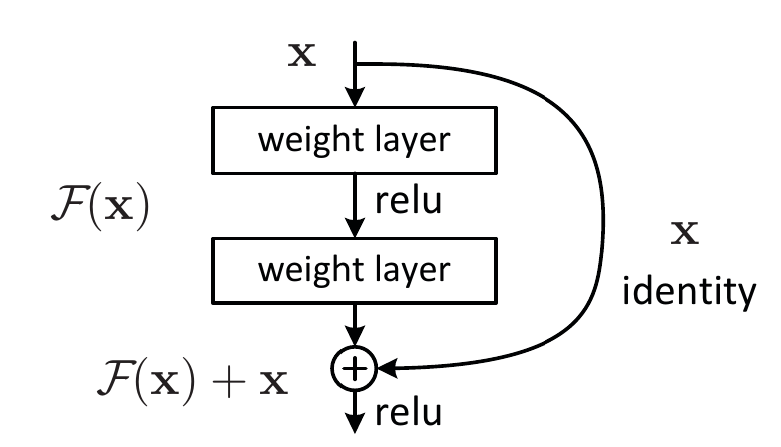
\includegraphics[width=0.7\linewidth]{resb1}
	\caption{نمونه ای از یک بلاک چسبنده. دقت کنید که چطور $\mathbf{x}$ یک میان‌بر مستقیم در شبکه دارد که دو لایه وزنی را پرش می‌کند.}
	\label{fig:resb1}
\end{figure}


\subsection{توابع فعال‌سازی}
توابع فعال‌سازی%
\LTRfootnote{Activation Functions}
در شبکه‌های عصبی برای ایجاد ویژگی‌های غیرخطی در مدل‌ها استفاده می‌شوند. این توابع به شبکه این امکان را می‌دهند که روابط پیچیده و غیرخطی بین ورودی‌ها و خروجی‌ها را یاد بگیرد و مدل‌هایی با قدرت تصمیم‌گیری بالا بسازد. بدون توابع فعال‌سازی، شبکه‌های عصبی فقط می‌توانند توابع خطی را مدل‌سازی کنند، که توانایی محدودی در پردازش داده‌های پیچیده دارند. انواع مختلفی از توابع فعال‌سازی وجود دارند، مانند تابع سیگموید (\lr{Sigmoid})، تانژانت هایپربولیک (\lr{Tanh})، \lr{ReLU} و \lr{GELU}، که هرکدام ویژگی‌های خاص خود را دارند. انتخاب تابع مناسب بستگی به ویژگی‌های داده‌ها و نوع مدل دارد، و استفاده صحیح از این توابع می‌تواند باعث بهبود عملکرد و همگرایی سریع‌تر مدل شود.


\subsubsection{سیگموید}
تابع فعال‌سازی سیگموید%
\LTRfootnote{Sigmoid Function}
یکی از توابع فعال‌سازی کلاسیک است که به‌طور گسترده در شبکه‌های عصبی به‌ویژه در مدل‌های لایه خروجی برای مسائل دسته‌بندی باینری استفاده می‌شود. این تابع مقادیر ورودی را به بازه $(0, 1)$ نگاشت می‌کند، که آن را برای مدل‌سازی احتمالات مفید می‌سازد. تابع سیگموید برای هر ورودی $x$ به‌صورت زیر تعریف می‌شود:
$$
\sigma(x) = \frac{1}{1 + e^{-x}}
$$
از ویژگی‌های مهم سیگموید می‌توان به قابلیت مشتق‌پذیری و شیب یکنواخت آن در تمام دامنه اشاره کرد. با این حال، سیگموید با مشکل محوشدگی گرادیان مواجه است، که زمانی رخ می‌دهد که مقادیر ورودی بسیار بزرگ یا کوچک باشند و باعث می‌شود که گرادیان‌ها به‌طور مؤثر صفر شوند، که فرآیند آموزش را کند می‌کند. علاوه بر این، سیگموید به دلیل محدودیت در بازه خروجی، در مسائل با خروجی‌های چندکلاسه یا مقادیر بزرگتر از 1 کاربرد کمتری دارد. باوجود این، سیگموید هنوز در بسیاری از مدل‌های عصبی به‌ویژه در لایه‌های خروجی برای پیش‌بینی احتمالات یا در مسائل دسته‌بندی باینری استفاده می‌شود.

\subsubsection{ReLU}
تابع فعال‌سازی ReLU%
\LTRfootnote{Rectified Linear Unit}
یکی از پرکاربردترین توابع در شبکه‌های عصبی مدرن است. این تابع ویژگی‌های غیرخطی را به مدل اضافه می‌کند و به‌طور ساده، مقادیر ورودی منفی را صفر کرده و مقادیر مثبت را بدون تغییر عبور می‌دهد. ReLU برای هر ورودی $x$ به‌صورت زیر تعریف می‌شود:
$$
\text{ReLU}(x) = \max(0, x)
$$
استفاده از ReLU باعث تسریع فرآیند آموزش می‌شود زیرا که محاسبات آن ساده و سریع است. علاوه بر این، ReLU به‌طور مؤثری از مشکل محو شدن گرادیان که در توابع فعال‌سازی کلاسیک‌تر مانند سیگموید یا تانژانت هایپربولیک مشاهده می‌شود، جلوگیری می‌کند. با این حال، یکی از معایب ReLU این است که ممکن است برخی از نورون‌ها به‌طور دائمی غیرفعال شوند، که به آن «مرگ نورون» گفته می‌شود. با این حال، انواعی از ReLU مانند \lr{Leaky ReLU} و \lr{Parametric ReLU} برای حل این مشکل پیشنهاد شده‌اند.


\subsubsection{GELU}
تابع GELU%
\LTRfootnote{Gaussian Error Linear Unit}
یک تابع فعال‌سازی که در ترنسفورمر ها به وفور استفاده می‌شود.  این تابع فعال‌سازی ویژگی‌های مفیدی از توابع غیرخطی دیگر مانند ReLU را حفظ می‌کند، در حالی‌که از مشکلاتی مانند برش (clipping) که در ReLU وجود دارد، جلوگیری می‌کند. تابع GELU به‌طور پیوسته و نرم ورودی‌ها را فعال می‌کند و به مدل این امکان را می‌دهد تا به‌طور مؤثری از ویژگی‌های مثبت و منفی ورودی‌ها بهره ببرد. GELU برای هر ورودی $x$ به‌صورت زیر تعریف می‌شود:
$$
\text{GELU}(x) = 0.5x \left( 1 + \tanh\left( \sqrt{\frac{2}{\pi}}(x + 0.044715x^3) \right) \right)
$$

\textbf{توابع فعال‌سازی دیگری هم هر کدام با نقات قوت و ضعف خود وجود دارند و استفاده می‌شوند که ما از توضیح آن‌ها صرفنظر می‌کنیم.}



\section{روش های ارزیابی}

ارزیابی عملکرد مدل‌های ترمیم تصویر یکی از مراحل حیاتی در توسعه و بهبود این سیستم‌ها است. از آنجا که ترمیم تصویر یک مسئله پیچیده و چندبعدی است، ارزیابی کیفی (مانند مشاهده بصری نتایج) به تنهایی نمی‌تواند معیار دقیقی برای مقایسه روش‌های مختلف ارائه دهد. همچنین این چالش وجود دارد که در سناریو های ارزیابی که در آن ها تصاویر زمینه حقیقت (GT) وجود ندارند، عمل «تشخیص ترمیم بهتر» موضوعی سلیقه ای می‌شود. در اینجا، معیارهای کمی (Quantitative) به عنوان ابزاری ضروری برای سنجش عینی عملکرد مدل‌ها مطرح می‌شوند. این معیارها امکان مقایسه سیستماتیک و دقیق بین روش‌های مختلف را فراهم می‌کنند و به پژوهشگران کمک می‌کنند تا نقاط قوت و ضعف هر روش را به‌طور علمی تحلیل کنند.
\subsection{معیار PSNR}
معیار PSNR (نسبت سیگنال به نویز پیک) رابطه‌ای است بین انرژی حداکثری یک سیگنال و نویزی که بر دقت نمایش آن تأثیر می‌گذارد. هرچه مقدار PSNR بالاتر باشد، کیفیت تصویر ترمیم‌شده بهتر خواهد بود.

برای محاسبه PSNR یک تصویر آزمایشی (g) با استفاده از تصویر مرجع (f)، ابتدا نیاز است که میانگین مربعات خطا (MSE) محاسبه شود. این مقدار از طریق معادله زیر به دست می‌آید:

\[
MSE = \frac{1}{N} \sum_{i=1}^{N} (f_i - g_i)^2
\]

که در آن $f_i$ و $g_i$ به ترتیب مقدار پیکسل‌های تصویر مرجع و تصویر آزمایشی هستند و $N$ تعداد کل پیکسل‌ها می‌باشد. پس از محاسبه MSE، مقدار PSNR به‌صورت زیر محاسبه می‌شود:

\begin{equation}
	PSNR = 10 \cdot \log_{10}\left(\frac{MAX^2}{MSE}\right)
\end{equation}

در اینجا $MAX$ مقدار حداکثری شدت پیکسل‌ها در تصویر است (برای تصاویر 8 بیتی معمولاً برابر با 255 است). PSNR معیاری برای ارزیابی کیفیت تصویر است که هرچه مقدار آن بیشتر باشد، به معنای کیفیت بالاتر تصویر ترمیم‌شده است.

\subsection{معیار SSIM}

SSIM
(شاخص مشابهت ساختاری) یک تکنیک برای اندازه‌گیری مشابهت بین دو تصویر است. این روش یک تصویر با کیفیت کامل را با تصویر دیگری (مثلا تصویر ترمیم شده) مقایسه می‌کند. این معیار توانایی مدل در حفظ ساختار و ویژگی‌های تصویر اصلی را اندازه‌گیری می‌کند.

مقادیر کوچک SSIM نشان‌می دهد تصویر ترمیم‌شده از تصویر مرجع تفاوت دارد. این مقادیر پایین به‌ویژه در نواحی آسیب‌دیده یا ترمیم‌شده مشاهده می‌شوند که در آن‌ها مدل نتوانسته است جزئیات تصویر اصلی را به‌خوبی بازسازی کند. برعکس، مقادیر بزرگ SSIM در نواحی یکنواخت تصویر مرجع مشاهده می‌شود، جایی که تصویر ترمیم‌شده مشابه تصویر اصلی است و تفاوت‌های کمی بین آن‌ها وجود دارد.

فرمول کلی SSIM به صورت زیر است:
$$
SSIM(f, g) = l(f, g) \cdot c(f, g) \cdot s(f, g)
$$

که در آن $l(f, g)$، $c(f, g)$ و $s(f, g)$ به ترتیب مولفه‌های روشنایی (luminance)، کنتراست (contrast) و ساختار (structure) هستند. این مولفه‌ها به شرح زیر تعریف می‌شوند:

\textbf{مولفه روشنایی}%
\LTRfootnote{Luminance}
: این مولفه تفاوت میانگین شدت روشنایی بین دو تصویر را اندازه‌گیری می‌کند. اگر میانگین شدت روشنایی تصویر مرجع ($\mu_f$) و تصویر ترمیم‌شده ($\mu_g$) نزدیک به هم باشند، مقدار $l(f, g)$ به 1 نزدیک می‌شود، که نشان‌دهنده شباهت بالا در روشنایی کلی است.
$$
l(f, g) = \frac{2\mu_f \mu_g + C_1}{\mu_f^2 + \mu_g^2 + C_1}
$$
که در آن $\mu_f$ و $\mu_g$ میانگین پیکسل‌های تصویر مرجع و تصویر ترمیم‌شده هستند، و $C_1$ یک مقدار ثابت کوچک برای جلوگیری از تقسیم بر صفر است.

\textbf{مولفه کنتراست}%
\LTRfootnote{Contrast}
:    این مولفه تغییرپذیری شدت پیکسل‌ها را در هر تصویر مقایسه می‌کند. اگر انحراف معیار ($\sigma_f$ و $\sigma_g$) دو تصویر مشابه باشند، مقدار $c(f, g)$ به 1 نزدیک می‌شود، که نشان می‌دهد کنتراست (تفاوت بین روشن‌ترین و تاریک‌ترین نواحی) در هر دو تصویر مشابه است.
$$
c(f, g) = \frac{2\sigma_f \sigma_g + C_2}{\sigma_f^2 + \sigma_g^2 + C_2}
$$
که در آن $\sigma_f$ و $\sigma_g$ انحراف معیار پیکسل‌های تصویر مرجع و تصویر ترمیم‌شده هستند، و $C_2$ مقدار ثابتی مشابه $C_1$ است.

\textbf{مولفه ساختار}
: این مولفه شباهت ساختاری بین دو تصویر را ارزیابی می‌کند. ساختار به رابطه بین پیکسل‌ها و همبستگی آن‌ها با یکدیگر اشاره دارد. اگر تصاویر مرجع و ترمیم‌شده دارای الگوهای ساختاری مشابه باشند (مثلاً در لبه‌ها و جزئیات)، مقدار $s(f, g)$ به 1 نزدیک خواهد بود.
$$
s(f, g) = \frac{\sigma_{fg} + C_3}{\sigma_f \sigma_g + C_3}
$$
که در آن $\sigma_{fg}$ همبستگی میان تصویر مرجع و تصویر ترمیم‌شده است، و $C_3$ مقدار ثابت دیگری برای جلوگیری از تقسیم بر صفر است.

ترکیب این سه مؤلفه از طریق ضرب آن‌ها تضمین می‌کند که SSIM تنها در صورتی مقدار بالایی خواهد داشت که تصاویر از نظر روشنایی، کنتراست و ساختار به یکدیگر بسیار شبیه باشند.

SSIM
به طور کلی به‌عنوان یک معیار بهتر از PSNR در ارزیابی کیفیت بصری تصویر شناخته می‌شود، چرا که SSIM قادر است ویژگی‌های بصری و ساختاری تصویر را با دقت بیشتری مدل‌سازی کند و علاوه بر اندازه‌گیری خطاهای نقطه‌ای، به ویژگی‌های ساختاری تصویر نیز توجه می‌کند و می‌تواند اطلاعات بیشتری در مورد شباهت‌های بصری بین دو تصویر ارائه دهد. این ویژگی به‌ویژه در ارزیابی تصاویر ترمیم‌شده که ممکن است خطاهای محلی داشته باشند، مفید است.



این تحلیل ها نشان می‌دهد که ترمیم تصویر یک مسئله پیچیده و چندوجهی است و می‌تواند به‌طور پیوسته از بازسازی محلی به سمت تولید کلی تصویر تغییر کند. در فصل بعدی، به بررسی کارهای پیشین در این حوزه می‌پردازیم و روش‌های کلیدی و پیشرفت‌های اخیر در ترمیم تصویر را مرور خواهیم کرد. این مرور به درک بهتر چالش‌ها و راه‌حل‌های موجود کمک می‌کند و زمینه را برای معرفی روش‌های نوین در فصل‌های بعدی فراهم می‌سازد.

%
\chapter{مطالعات پیشین}

در این فصل، به مرور مطالعات پیشین و روش‌های مرتبط ترمیم تصویر پرداخته می‌شود. هدف از این مرور، شناسایی نقاط قوت و ضعف روش‌های موجود، بررسی پیشرفت‌های اخیر در حوزه مرتبط، بررسی مجموعه‌داده های ترمیم تصویر و ارائه پیش‌زمینه ای از متدولوژی های مرسوم ترمیم است.

ابتدا به بررسی تاریخچه و پیشرفت روش‌های مرتبط با ترمیم تصاویر پرداخته خواهد شد و دسته‌بندی‌های مختلف این روش‌ها، به همراه مزایا و معایب آن‌ها مورد بحث قرار خواهد گرفت. سپس، مجموعه داده‌های مورد استفاده در این حوزه معرفی شده و معیارهای مورد نظر برای ارزیابی این روش‌ها توضیح داده می‌شوند. در نهایت، الگوریتم‌های کلاسیک و روش‌های مبتنی بر یادگیری عمیق که تاکنون برای ترمیم تصاویر پیشنهاد شده‌اند، بررسی خواهند شد. این تحلیل به عنوان مبنایی برای توجیه ضرورت استفاده از معماری ترنسفورمر در تحقیق حاضر خواهد بود.

\section{روش های الگوریتمی}

مسئله ترمیم تصویر به قبل‌تر از ظهور روش‌های مبتنی بر یادگیری عمیق بازمی‌گردد. در ابتدا این مسئله به کمک روش‌های الگوریتمی کلاسیک مورد بررسی قرار گرفت. یکی از اولین روش‌های مطرح‌شده در حوزه ترمیم تصاویر، رویکرد مبتنی بر انتشار بود که توسط Bertalmio و همکارانش در سال ۲۰۰۰ معرفی شد \cite{bertalmioImageInpainting2000}. این روش از معادلات دیفرانسیل جزئی \lr{(PDE)} برای گسترش اطلاعات موجود در لبه‌های تصویر به نواحی آسیب‌دیده استفاده می‌کند. ایده اصلی این روش، شبیه‌سازی فرآیند طبیعی انتشار اطلاعات در تصویر است تا ساختارهای محلی به صورت پیوسته بازسازی شوند. با وجود اینکه این روش برای ترمیم نواحی کوچک و حفظ ساختار لبه‌ها عملکرد خوبی دارد، اما روشی ابتدایی مبتنی بر محلی ترین مفروضات تصویر بوده و در بازسازی نواحی بزرگ‌تر یا بافت‌های پیچیده به دلیل محدودیت درک محتوای کلی تصویر ناکارآمد است.

در ادامه رویکردهای مبتنی بر انتشار، روش ترمیم تصویر با تغییرات کل \lr{(Total Variation Inpainting)} که توسط Chan و Shen در سال ۲۰۰۱ معرفی شد \cite{chanNontextureInpaintingCurvatureDriven2001}، گامی دیگر در پیشرفت این حوزه بود. این روش بر مبنای به حداقل رساندن یک تابع انرژی طراحی شده است که هدف آن حفظ ساختار لبه‌ها و جلوگیری از ایجاد تاری در نواحی بازسازی‌شده است. مدل تغییرات کل از معادلات دیفرانسیل جزئی برای انتقال اطلاعات لبه‌ها به نواحی آسیب‌دیده استفاده می‌کند و توانایی بالایی در بازسازی ساختارهای ساده دارد. با این حال، مانند روش Bertalmio و همکاران، این رویکرد نیز در بازسازی بافت‌های پیچیده یا نواحی بزرگ با محدودیت‌هایی مواجه است.


دسته دیگری از روش‌های کلاسیک که به مراتب موفق تر عمل کردند، روش‌های مبتنی بر وصله \lr{(Patch-Based Methods)} بودند. در این روش‌ها، نواحی سالم تصویر به عنوان بانک وصله‌ها در نظر گرفته می‌شدند و بهترین تطابق برای پر کردن نواحی آسیب‌دیده از میان این وصله‌ها انتخاب می‌شد.

به‌عنوان مثال در یکی از برجسته ترین روش های غیرمبتنی بر یادگیری، بارنز و همکاران در \cite{barnesPatchMatchRandomizedCorrespondence2009} با معرفی PatchMatch ابزارهای تعاملی ویرایش تصویر را با استفاده از یک الگوریتم تصادفی جدید ارائه داده‌اند که امکان یافتن بسیار سریع تطابق‌های تقریبی نزدیک‌ترین همسایه بین قطعات تصویر را فراهم می‌کند. الگوریتم ارائه‌شده توسط آن‌ها بهبودهای قابل‌توجهی در عملکرد نسبت به روش‌های پیشین (۲۰ تا ۱۰۰ برابر سریع‌تر) ارائه می‌دهد و استفاده از آن را در ابزارهای تعاملی ممکن می‌سازد. بینش‌های کلیدی این الگوریتم شامل یافتن برخی تطابق‌های مناسب از طریق نمونه‌گیری تصادفی و استفاده از هم‌بستگی طبیعی در تصاویر برای انتشار سریع این تطابق‌ها به نواحی مجاور است.

با وجود این که این رویکردها توانستند نتایج بهتری نسبت به روش های مبتنی بر PDE در بازسازی جزئیات ارائه دهند، اما به دلیل تکیه بر ویژگی‌های محلی و وابستگی به مشابهت بافتی، در مواجهه با تصاویر پیچیده و متنوع محدودیت‌های زیادی داشتند و اکثرا مفروضات عمیقی در مورد تصاویر هدفشان داشتند. یکی از این مفروضات، فرض رنک پایین بودن تصاویر است. این فرض بر این ایده استوار است که داده‌های تصویری در بسیاری از کاربردها، به‌ویژه در تصاویر طبیعی، به صورت ذاتی دارای ساختار رنک پایین هستند. به این معنا که اطلاعات موجود در یک تصویر را می‌توان در یک فضای برداری با ابعاد بسیار کمتر نسبت به فضای اصلی بازنمایی کرد. روش‌های مبتنی بر این فرض، مانند تجزیه مقدار منفرد \lr{(SVD)}
\cite{yaghmaeeImprovingImageInpainting2020}
 و فشرده‌سازی رنک پایین، در بسیاری از مسائل پردازش تصویر نظیر ترمیم تصویر، کاهش نویز و فشرده‌سازی داده به کار گرفته شدند. با این حال، این الگوریتم‌های کلاسیک اغلب در شرایط پیچیده‌تر مانند تصاویر با ساختار غیرخطی، نواحی هدف ترمیم بسیار بزرگ، نواحی بافت‌های پیچیده، یا تصاویر آسیب‌دیده با نویز بالا عملکرد ضعیفی داشتند. این محدودیت‌ها ناشی از این واقعیت است که تصاویر واقعی معمولاً از روابط غیرخطی پیچیده و وابستگی‌های بلندمدت میان پیکسل‌ها پیروی می‌کنند که فرض رنک پایین قادر به مدل‌سازی آن‌ها نیست. علاوه بر این، این روش‌ها اغلب فرض می‌کنند که اطلاعات کلیدی تصویر به صورت یکنواخت توزیع شده است، در حالی که در واقعیت، اطلاعات تصاویر در نواحی مختلف دارای توزیع‌های بسیار متفاوتی است.
 
 همچنین در ترمیم تصاویر با نواحی هدف ماسک شده بسیار بزرگ، روش های مبتنی بر وصله نیازمند وصله هایی مشابه در تصویر بودند تا با استفاده از آن ها، نواحی مورد نظر را ترمیم کنند. فرض استوار این روش ها بر این بود که برای هر تصویر $I$ شامل وصله‌هایی مانند $x = \{x_1, x_2, \dots, x_n\}$ است که می‌توانند از طریق ترکیب یا تبدیل‌های خطی و غیرخطی، ویژگی‌های معنایی دقیقی را برای بازسازی نواحی گمشده تولید کنند. به بیان ریاضی، این فرضیه به این معناست که برای هر وصله گمشده $x_{\text{missing}}$، می‌توان یک ترکیب بهینه از وصله‌های موجود $x_{\text{observed}}$ پیدا کرد که به صورت زیر بازسازی را انجام دهد:
 
 $$
 x_{\text{missing}} \approx \sum_{i=1}^{n} w_i \cdot T_i(x_i)
 $$


با این حال، با افزایش اندازه ماسک، یا ماسک کردن نواحی با الگو های پیچیده اما یکتا مانند چهره ها، این فرضیه دیگر معتبر نیست. در چنین حالتی، نواحی گمشده به‌حدی بزرگ هستند که وصله‌های مشابه کافی در تصویر وجود ندارد، یا ترکیب آن‌ها نمی‌تواند ویژگی‌های معنایی دقیق و نوآورانه مورد نیاز را تولید کند. در نتیجه، روش‌های مبتنی بر وصله نیز، در مواجهه با ماسک‌های بزرگ، به‌دلیل عدم توانایی در تولید ویژگی‌های معنایی جدید، با محدودیت مواجه می‌شوند.

\section{روش‌های مبتنی بر یادگیری عمیق}

با ظهور یادگیری عمیق و توانایی آن در استخراج ویژگی‌های پیچیده از داده‌های تصویری و همچنین تولید ویژگی های نوین لازم برای انواع چالش‌برانگیزی از مسائل ترمیم، پژوهش‌ها در زمینه ترمیم تصاویر به سمت استفاده از مدل‌های مبتنی بر شبکه‌های عصبی سوق یافت. این روش‌ها با استفاده از مجموعه داده‌های بزرگ و متنوع، قادر به یادگیری الگوهای پیچیده و بازسازی دقیق‌تر نواحی آسیب‌دیده شدند. برخلاف روش‌های الگوریتمی که عمدتاً بر اصول ریاضی و آماری استوار بودند، روش‌های مبتنی بر یادگیری امکان درک مفاهیم سطح بالا و روابط سراسری در تصویر را فراهم کردند و موفق شدند ترمیم هایی با  ماسک های بزرگ‌تر انجام دهند، چرا که این امر گاها نیازمند ساخت ساختار های کاملا جدید در تصویر (مانند ساختار چهره، طبیعت و ...) بود. 

\section{مجموعه‌داده‌های ترمیم تصویر}

یکی از عوامل کلیدی در موفقیت مدل‌های یادگیری عمیق در پردازش تصویر، وجود مجموعه‌داده‌های بزرگ و متنوع است که امکان آموزش مدل‌ها در سناریوهای گوناگون را فراهم می‌سازد. مجموعه‌داده‌های مختلف برای کاربردهای خاص طراحی شده‌اند و هر یک ویژگی‌های منحصربه‌فردی دارند. در ادامه، به معرفی برخی از مجموعه‌داده‌های شناخته‌شده مانند \lr{CelebA-HQ}، \lr{Places}، و چندین مجموعه‌داده دیگر پرداخته می‌شود.


مجموعه‌داده \textbf{CelebA-HQ} یکی از معروف‌ترین مجموعه‌داده‌ها برای تحلیل چهره است. این مجموعه‌داده‌ی کلاس‌بندی نشده، شامل تصاویری با وضوح بالا از چهره انسان است که ویژگی‌هایی مانند موقعیت، حالت، رنگ پوست، زاویه و روشنایی های مختلف را پوشش می‌دهد. CelebA-HQ به‌طور گسترده در زمینه‌هایی مانند بازسازی تصویر، تغییر چهره، و شناسایی چهره استفاده شده است. ویژگی برجسته این مجموعه‌داده، کیفیت بالای تصاویر و پوشش گسترده از حالات و ویژگی‌های مختلف چهره است که آن را به انتخابی محبوب برای مدل‌های یادگیری عمیق تبدیل کرده است.

\begin{figure}
	\centering
	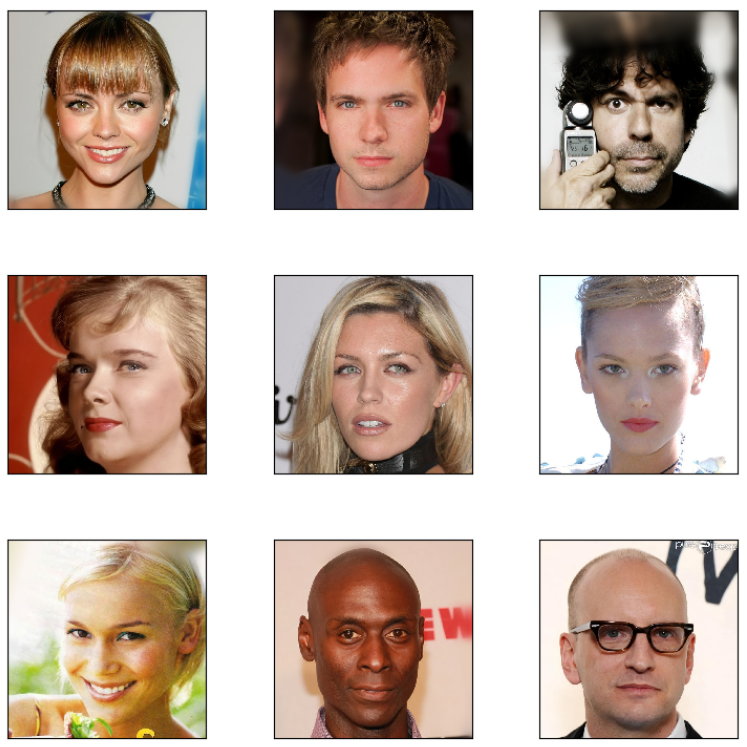
\includegraphics[width=0.7\linewidth]{celebahq1}
	\caption{نمونه تصاویر از مجموعه‌داده Celeb-A-HQ. تمرکز این دیتاست بر روی فیچر های چهره است.}
	\label{fig:celebahq1}
\end{figure}

مجموعه‌داده \textbf{Places} برای تحلیل صحنه‌ها و شناخت محیط‌ها طراحی شده است. این مجموعه‌داده‌ی کلاس‌بندی شده، شامل میلیون‌ها تصویر از محیط‌های مختلف مانند مناظر طبیعی، محیط‌های شهری، و فضاهای داخلی است. مجموعه Places برای کاربردهایی مانند تشخیص صحنه، طبقه‌بندی محیط، و تولید تصاویر صحنه استفاده می‌شود. یکی از ویژگی‌های کلیدی این مجموعه‌داده، تنوع بالا در دسته‌بندی‌های محیطی است که امکان آموزش مدل‌هایی با درک عمیق‌تر از صحنه‌های مختلف را فراهم می‌کند.

\begin{figure}
	\centering
	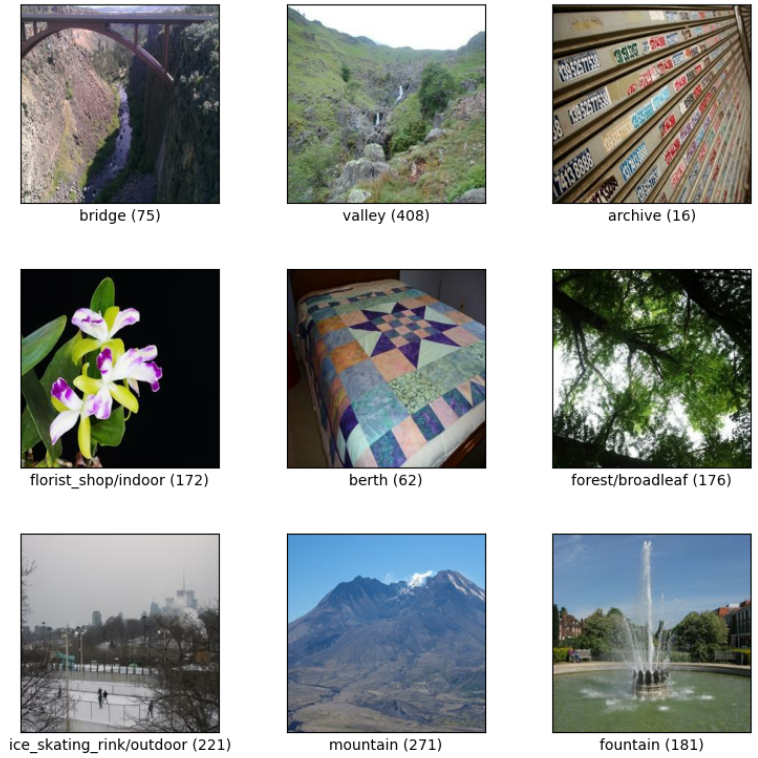
\includegraphics[width=0.7\linewidth]{places1}
	\caption{نمونه تصاویر از مجموعه‌داده Places به همراه یک کلمه برای توصیف هر تصویر و اندیس هر فایل در داخل پرانتز}
	\label{fig:places1}
\end{figure}


مجموعه‌داده \textbf{ImageNet} یکی از جامع‌ترین مجموعه‌داده‌های موجود در حوزه یادگیری عمیق است که با بیش از ۱۴ میلیون تصویر
\footnote{این مجموعه‌داده هر سال در حال بروزرسانی و افزوده شدن است. آمار ذکر شده آخرین آمار تا ژانویه ۲۰۲۵ است.}
در ۱۰۰۰ طبقه‌بندی مختلف تأثیر شگرفی بر پیشرفت شبکه‌های عصبی داشته است. ImageNet علاوه بر کاربردهای عمومی مانند طبقه‌بندی تصویر، به‌عنوان یک معیار استاندارد برای ارزیابی عملکرد مدل‌های یادگیری عمیق استفاده می‌شود. موفقیت‌های اولیه شبکه‌های عصبی کانولوشنی (CNN) مانند AlexNet و ResNet تا حد زیادی مرهون این مجموعه‌داده بزرگ و متنوع بوده‌اند.



%یکی دیگر از مجموعه‌داده‌های مهم، \textbf{MS-COCO} است که برای وظایف پیشرفته‌تری مانند تشخیص اشیا، بخش‌بندی تصویر، و توصیف تصویر طراحی شده است. این مجموعه‌داده شامل تصاویری است که حاوی چندین شیء از دسته‌بندی‌های مختلف هستند، و هر تصویر دارای برچسب‌های متنی دقیق و اطلاعات مربوط به موقعیت اشیاء است. MS-COCO به‌طور گسترده در مدل‌هایی که نیازمند درک پیچیده‌تر تصویر هستند، مانند مدل‌های تولید متن از تصویر
%\LTRfootnote{Image Captioning}
%یا سیستم‌های تشخیص چند‌شیء، استفاده می‌شود.
مجموعه داده
\lr{DTD (Describable Textures Dataset)}
یک مجموعه داده شامل $5640$ تصویر واقعی از بافت‌های مختلف است که با یک یا چند صفت توصیفی از یک واژگان ۴۷ کلمه‌ای در زبان انگلیسی برچسب‌گذاری شده‌اند. این مجموعه داده به‌طور خاص برای مطالعه و تحلیل بافت‌های قابل توصیف طراحی شده است و شامل نمونه‌هایی از بافت‌های طبیعی و مصنوعی است. 

از ویژگی‌های قابل توجه \lr{DTD} می‌توان به تنوع گسترده تصاویر و برچسب‌های توصیفی دقیق اشاره کرد که آن را به یک منبع ارزشمند در کاربردهایی نظیر دسته‌بندی بافت‌ها، تشخیص الگو و آموزش مدل‌های یادگیری عمیق تبدیل کرده است. این مجموعه داده برای ارزیابی مدل‌های بینایی کامپیوتر که نیاز به درک ویژگی‌های بصری بافت‌ها دارند، به‌ویژه در مسائل مرتبط با توصیف و دسته‌بندی، بسیار مناسب است.

در جدول \ref{tab:datasets_summary} خلاصه ای از مجموعه‌داده های بیان‌شده آورده شده است.
\warningToSelfExpandable

\begin{figure}
	\centering
	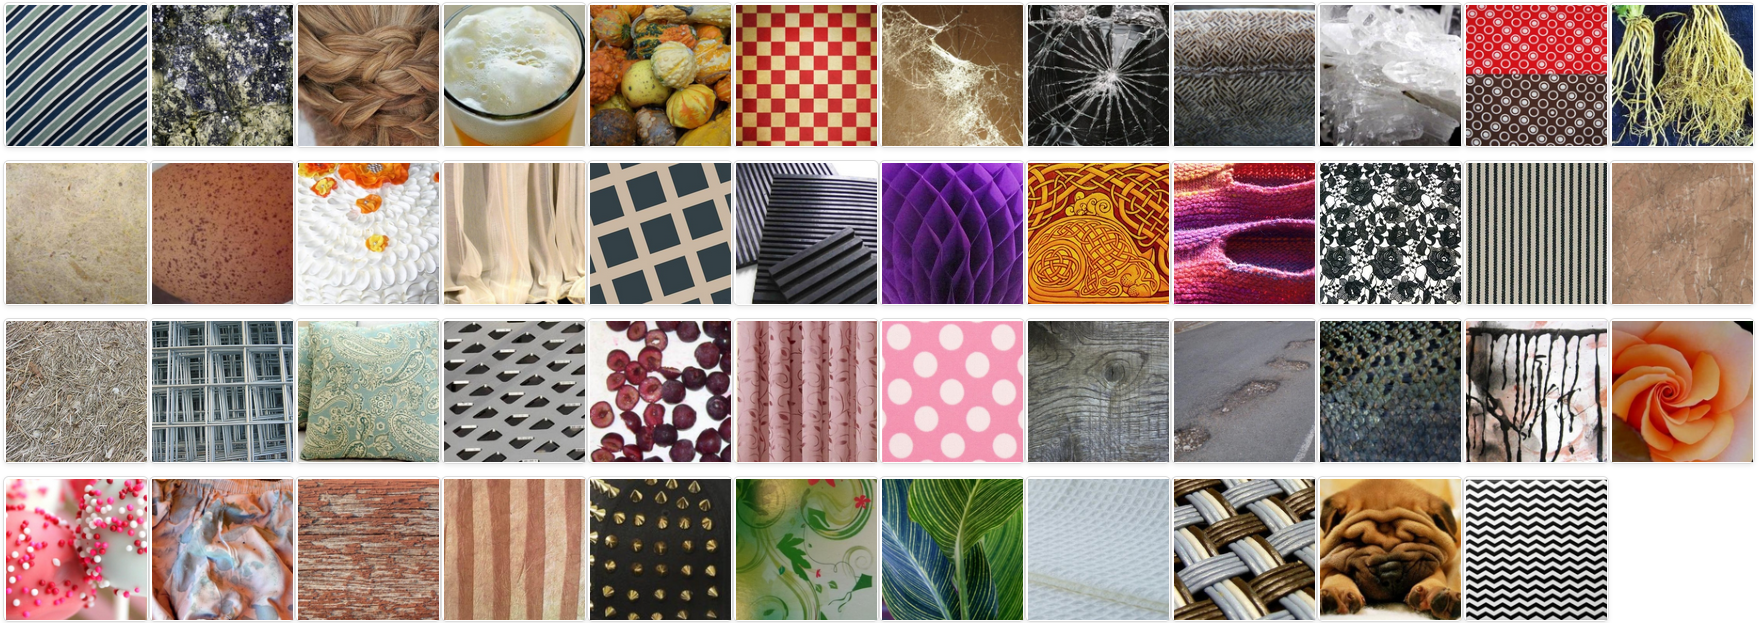
\includegraphics[width=0.7\linewidth]{dtd1}
	\caption{نمونه تصاویر مجموعه‌داده DTD}
	\label{fig:dtd1}
\end{figure}



\begin{table}
	\centering
	\label{tab:datasets_summary}
	\begin{tabular}{|l|c|c|l|}
		\hline
		\textbf{نام مجموعه داده} & \textbf{برچسب‌دار (بله/خیر)} & \textbf{تعداد تصاویر} & \textbf{ویژگی} \\ \hline
		\lr{Places2} \cite{zhouPlacesImageDatabase2016} & بله & $>10,000,000$ & محیط‌ها \\ \hline
		\lr{CelebA} \cite{liuDeepLearningFace2015} & بله & $200,000$ & چهره \\ \hline
		\lr{CelebHQ} \cite{karrasProgressiveGrowingGANs2018} & بله & $30,000$ & چهره با کیفیت \\ \hline
		\lr{DTD} \cite{cimpoiDescribingTexturesWild2013} & بله & $5,640$ & بافت \\ \hline
		\lr{ImageNet} \cite{russakovskyImageNetLargeScale2015} & بله &  $>14,000,000$
		\tablefootnote{این مجموعه‌داده هر سال در حال بروزرسانی و افزوده شدن است. آمار ذکر شده آخرین آمار تا ژانویه ۲۰۲۵ است.}
		 & اشیاء \\ \hline
	\end{tabular}
	\caption{خلاصه‌ای از مجموعه داده‌های معروف}
\end{table}


\begin{figure}
	\centering
	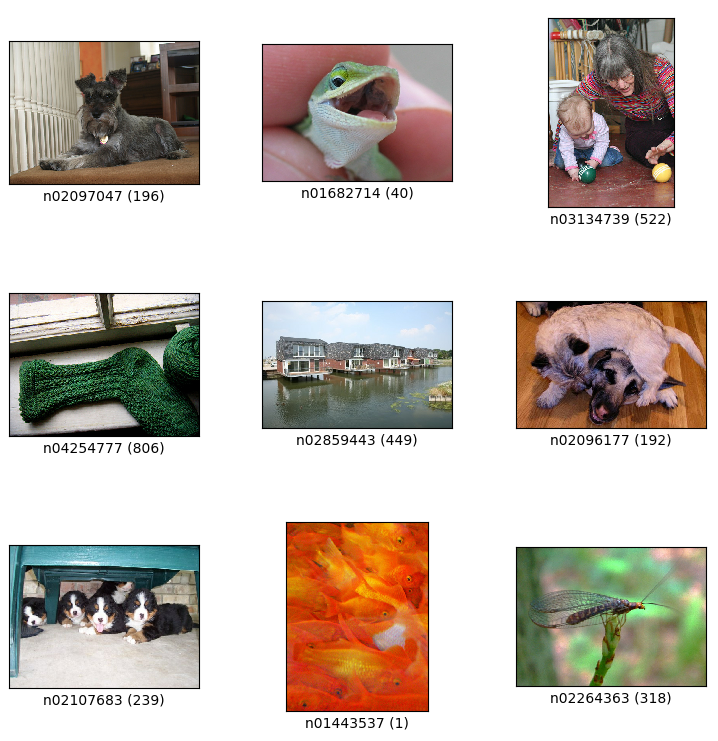
\includegraphics[width=0.7\linewidth]{imagenet2012-1}
	\caption{نمونه تصاویر از مجموعه‌داده
		ImageNet
		نسخه سال ۲۰۱۲ به همراه یک کلمه برای توصیف هر تصویر و نام هر فایل در داخل پرانتز}
	\label{fig:imagenet2012-1}
\end{figure}


\section{روش های مبتنی بر کانولوشن}

Pathak
و همکاران در \cite{pathakContextEncodersFeature2016}
یک الگوریتم یادگیری ویژگی‌های بصری بدون نظارت \LTRfootnote{Unsupervised} ارائه داده‌اند که بر اساس پیش‌بینی پیکسل مبتنی بر زمینه هدایت می‌شود. به‌طور مشابه با خودرمزگذارها
\LTRfootnote{Autoencoders}
، آن‌ها کدگذاران زمینه (\lr{Context Encoders}) را پیشنهاد کرده‌اند – یک شبکه عصبی کانولوشنی که برای تولید محتوای یک ناحیه دلخواه از تصویر، با توجه به محیط اطراف آن آموزش داده شده است. برای موفقیت در این وظیفه، معماری پیشنهادی باید هم محتوای کل تصویر را درک کنند و هم فرضیه‌ای معقول برای قسمت‌های حذف‌شده ارائه دهند.  

آن‌ها در فرایند آموزش کدگذار زمینه، از دو رویکرد استفاده کرده‌اند: یکی اتکای صرف به تابع هزینه بازسازی پیکسل-محور استاندارد بر اساس نرم دوم (\lr{L2 Loss})، و دیگری ترکیب بازسازی با یک تابع هزینه رقابتی (\lr{Adversarial Loss}) پیشنهاد شده در شبکه های GAN
\cite{goodfellowGenerativeAdversarialNetworks2014}.
نتایج نشان داده است که رویکرد دوم خروجی‌هایی با وضوح بالاتر تولید می‌کند، زیرا بهتر می‌تواند حالت‌های چندگانه در خروجی را مدیریت کند. "حالت‌های چندگانه" به این معناست که برای یک ناحیه گمشده در تصویر، چندین امکان معنایی و بصری معتبر برای پر کردن آن وجود دارد. به عبارت دیگر، ناحیه گمشده می‌تواند به‌طور همزمان با محتوای مختلفی که همگی با زمینه تصویر سازگار هستند، پر شود. این موضوع به دلیل تعدد راه‌حل‌های ممکن در مسئله ترمیم تصویر رخ می‌دهد.\\


\begin{table}[h!]
	\centering
	\begin{tabular}{|c|c|c|c|}
		\hline
		\textbf{روش} & \textbf{\lr{L1} میانگین} & \textbf{\lr{L2} میانگین} & \textbf{\lr{PSNR} (بالاتر بهتر)} \\ \hline
		\lr{NN-inpainting (HOG)} \cite{haysSceneCompletionUsing2007} & \lr{19.92\%} & \lr{6.92\%} & \lr{12.79 dB} \\ \hline
		\lr{NN-inpainting} (بردار ویژگی‌های کدگذار زمینه) & \lr{15.10\%} & \lr{4.30\%} & \lr{14.70 dB} \\ \hline
		کدگذار زمینه (ترکیبی) & \lr{09.37\%} & \lr{1.96\%} & \lr{18.58 dB} \\ \hline
	\end{tabular}
	\caption{مقایسه روش‌ کدگذار زمینه با روش های دیگر بر اساس \lr{L1} میانگین، \lr{L2} میانگین و \lr{PSNR} روی مجموعه‌داده خیابان های پاریس.}
	\label{tab:context_encoders_inpainting_results}
\end{table}


\begin{figure}
	\centering
	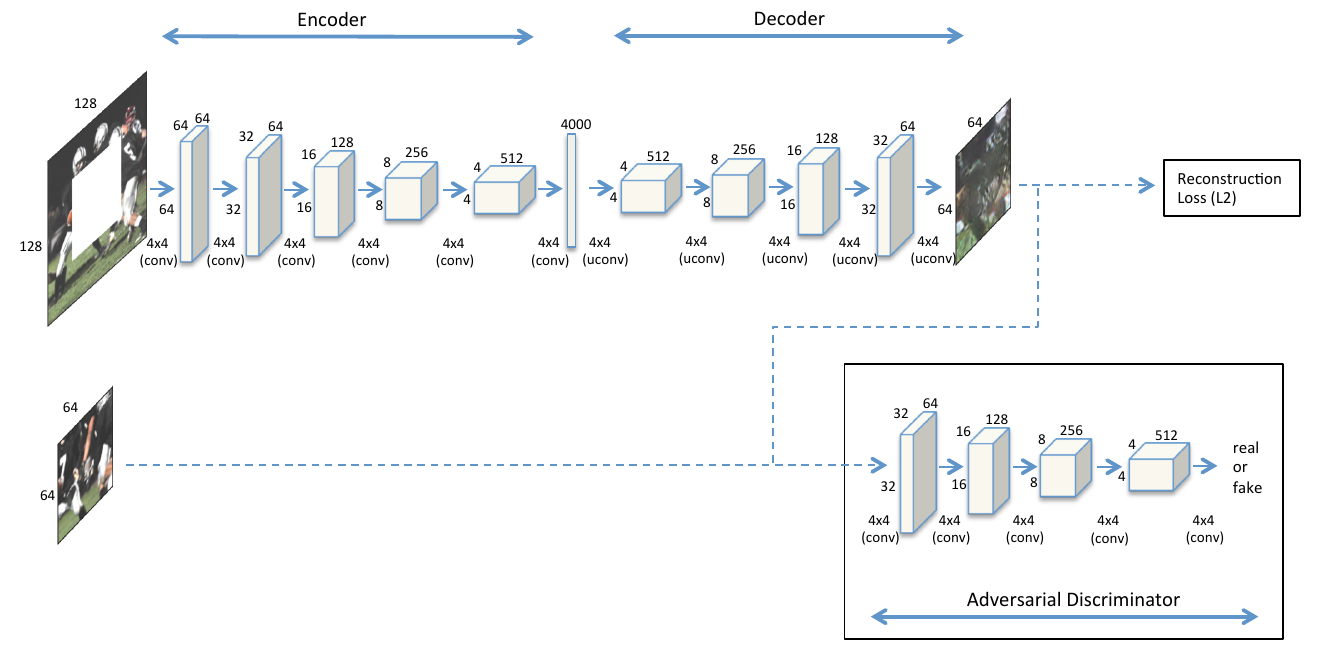
\includegraphics[width=1\linewidth]{pathakGanArch}
	\caption{معماری کدگذار زمینه که با ترکیب توابع هزینه بازسازی و رقابتی برای ترمیم معنایی آموزش دیده است.}
	\label{fig:pathakganarch}
\end{figure}



\begin{figure}
	\centering
	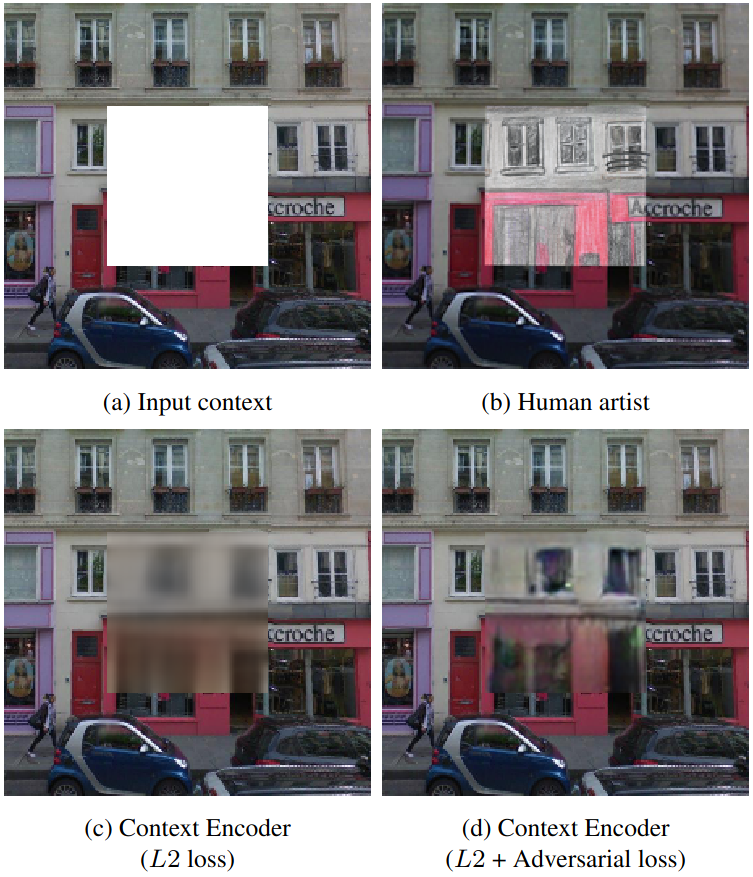
\includegraphics[width=0.7\linewidth]{figs/contextencodersLossComparison}
	\caption{مقایسه کیفی  استفاده از تابع هزینه نرم  ۲ در مقابل استفاده از یک تابع هزینه رقابتی در خروجی های تولید شده. 
		(a) عکس ورودی با یک قسمت از دست رفته 
		(b) یک انسان هنرمند مشکلی در ترمیم این تصویر ندارد 
		(c)
ترمیم خودکار تصویر با استفاده از کدگذار زمینه که توسط تابع هزینه بازسازی بر اساس نرم ۲ آموزش داده شده است.
	(d)
ترمیم خودکار تصویر با استفاده از کدگذار زمینه که توسط تابع هزینه رقابتی آموزش داده شده است.
}
	\label{fig:contextencoderslosscomparison}
\end{figure}



آن‌ها دریافتند  کدگذارهای زمینه بازنمایی هایی یاد می‌گیرند که نه‌تنها ظاهر، بلکه معنای ساختارهای بصری را نیز در بر می‌گیرد. اثربخشی این ویژگی‌های یادگرفته‌شده به‌طور کمّی برای پیش‌آموزش شبکه‌های عصبی کانولوشنی در وظایف طبقه‌بندی، تشخیص و قطعه‌بندی نشان داده شده است. علاوه بر این، کدگذارهای زمینه می‌توانند برای وظایف ترمیم معنایی تصاویر مورد استفاده قرار گیرند، چه به‌صورت مستقل و چه به‌عنوان نقطه شروع برای روش‌های غیرپارامتری.
\begin{figure}
	\centering
	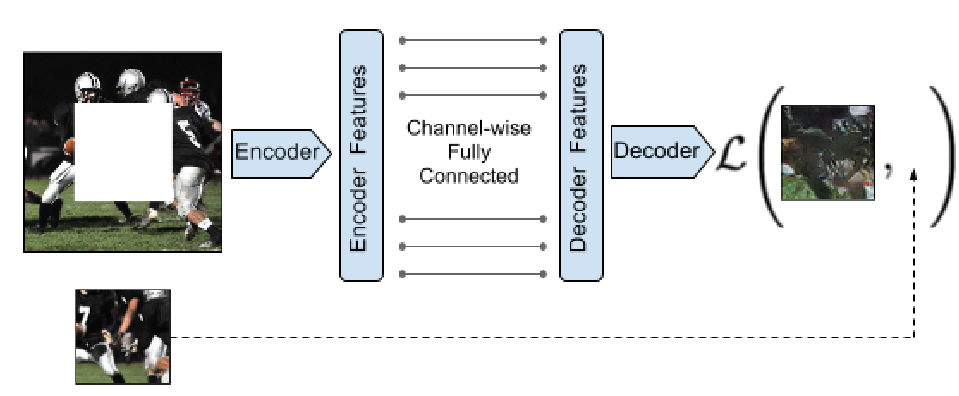
\includegraphics[width=0.7\linewidth]{figs/contextencodersArchitecture}
	\caption[معماری کلی Context Encoders]{
	تصویر زمینه از طریق بخش رمزگذار عبور داده می‌شود تا ویژگی‌هایی استخراج شوند که از طریق یک لایه کاملاً متصل کانال‌محور به رمزگشا متصل می‌شوند. سپس، رمزگشا نواحی حذف‌شده تصویر را تولید می‌کند.}
	\label{fig:contextencodersarchitecture}
\end{figure}

به دنبال این روش، روش های بسیاری بر پایه GAN ابداع شدند. 
\cite{caoLearningSketchTensor2021}
\cite{guoImageInpaintingConditional2024}
\cite{liRecurrentFeatureReasoning2020}
\cite{nazeriEdgeConnectGenerativeImage2019}
\cite{pengGeneratingDiverseStructure2021}

به عنوان مثال ایزُوکا و همکاران یک رویکرد نوین برای تکمیل تصویر ارائه دادند
\cite{iizukaGloballyLocallyConsistent2017}
که تصاویر به‌دست‌آمده هم از نظر محلی و هم از نظر سراسری سازگار بودند. با استفاده از یک شبکه عصبی کاملاً کانولوشنی، آن‌ها توانستند تصاویر با وضوح‌های دلخواه را با پر کردن نواحی گم‌شده به هر شکل تکمیل کنند. برای آموزش این شبکه تکمیل تصویر به‌طور سازگار، از متمایزکننده‌های بافت سراسری و محلی استفاده کردند که به‌طور خاص برای تشخیص تصاویر واقعی از تصاویر تکمیل‌شده آموزش دیده‌اند. متمایزکننده سراسری کل تصویر را بررسی می‌کند تا ارزیابی کند که آیا تصویر به‌طور کلی هماهنگ است یا نه، در حالی که متمایزکننده محلی فقط ناحیه‌ای کوچک متمرکز بر ناحیه تکمیل‌شده را بررسی می‌کند تا از سازگاری محلی وصله‌های تولیدشده اطمینان حاصل کند. سپس شبکه تکمیل تصویر برای فریب دادن هر دو شبکه متمایزکننده بافت آموزش داده می‌شود، که نیاز به تولید تصاویری دارد که از نظر سازگاری کلی و جزئیات با تصاویر واقعی غیرقابل تمایز باشند. این رویکرد نشان داد که می‌تواند برای تکمیل طیف وسیعی از صحنه‌ها استفاده شود. علاوه بر این، در مقایسه با رویکردهای مبتنی بر وصله مانند \lr{PatchMatch}، رویکرد آن‌ها می‌تواند تکه‌هایی تولید کند که در جای دیگری از تصویر ظاهر نمی‌شوند، که این امکان را می‌دهد که تصاویر اشیاء با ساختارهای آشنا و بسیار خاص، مانند صورت‌ها، به‌طور طبیعی تکمیل شوند.\\

\begin{table}[ht]
	\centering
	\begin{tabular}{|c|c|c|c|}
		\hline
		\textbf{} & \textbf{مبتنی بر وصله} & \textbf{کدگذار زمینه} & \textbf{ایزوکا و همکاران} \\
		\hline
		\textbf{اندازه تصویر} & \textbf{هر اندازه} & ثابت & \textbf{هر اندازه} \\
		\hline
		\textbf{سازگاری محلی} & \textbf{بله} & خیر & \textbf{بله} \\
		\hline
		\textbf{معناشناسی} & خیر & \textbf{بله} & \textbf{بله} \\
		\hline
		\textbf{اشیاء نوین} & خیر & \textbf{بله} & \textbf{بله} \\
		\hline
	\end{tabular}
	\caption{مقایسه روش‌ ارائه شده توسط ایزوکا  و همکاران در مقایسه با کدگذارهای زمینه و روش های الگوریتمی مبتنی بر وصله.}
\end{table}


\begin{figure}
	\centering
	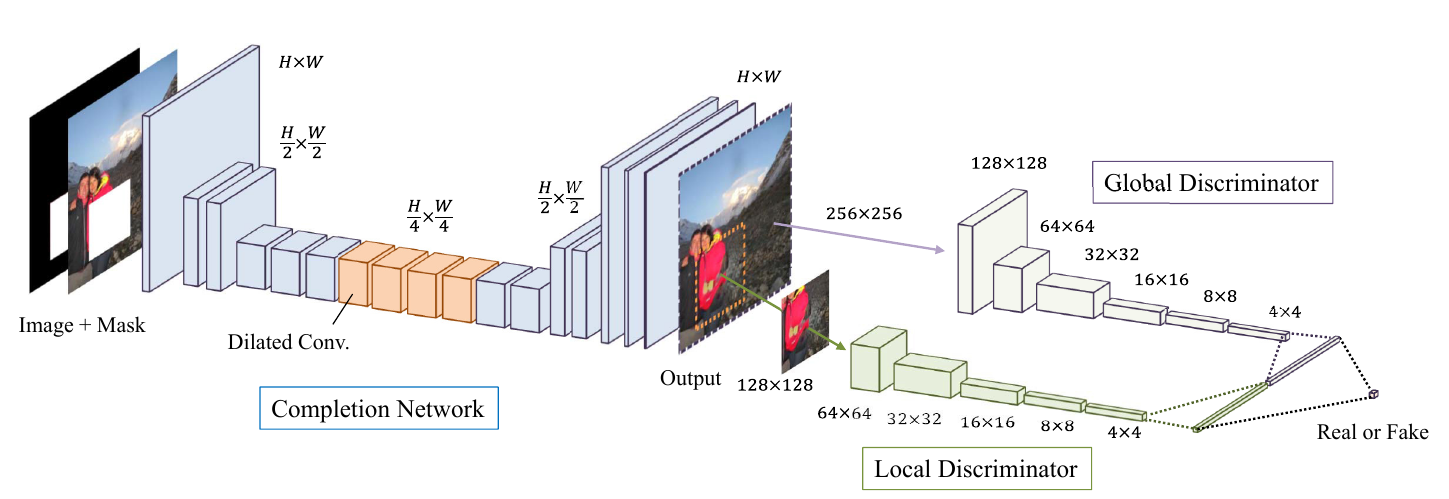
\includegraphics[width=1\linewidth]{IISUKAArch1}
	\caption{مروری بر معماری ایزوکا و همکاران برای یادگیری ترمیم تصویر. این معماری شامل یک شبکه تکمیل و دو شبکه متمایزکننده کمکی زمینه است که تنها برای آموزش شبکه تکمیل  کننده استفاده می‌شوند و در طول آزمایش (\lr{Inference})
		 مورد استفاده قرار نمی‌گیرند. شبکه متمایزکننده سراسری کل تصویر را به‌عنوان ورودی می‌گیرد، در حالی که شبکه متمایزکننده محلی تنها ناحیه‌ای کوچک اطراف ناحیه تکمیل‌شده را به‌عنوان ورودی می‌گیرد. هر دو شبکه متمایزکننده آموزش داده می‌شوند تا تشخیص دهند که آیا تصویر واقعی است یا توسط شبکه تکمیل‌کننده ساخته شده است، در حالی که شبکه تکمیل‌کننده برای فریب دادن هر دو شبکه متمایزکننده آموزش داده می‌شود.}
	\label{fig:iisukaarch1}
\end{figure}


\begin{figure}
	\centering
	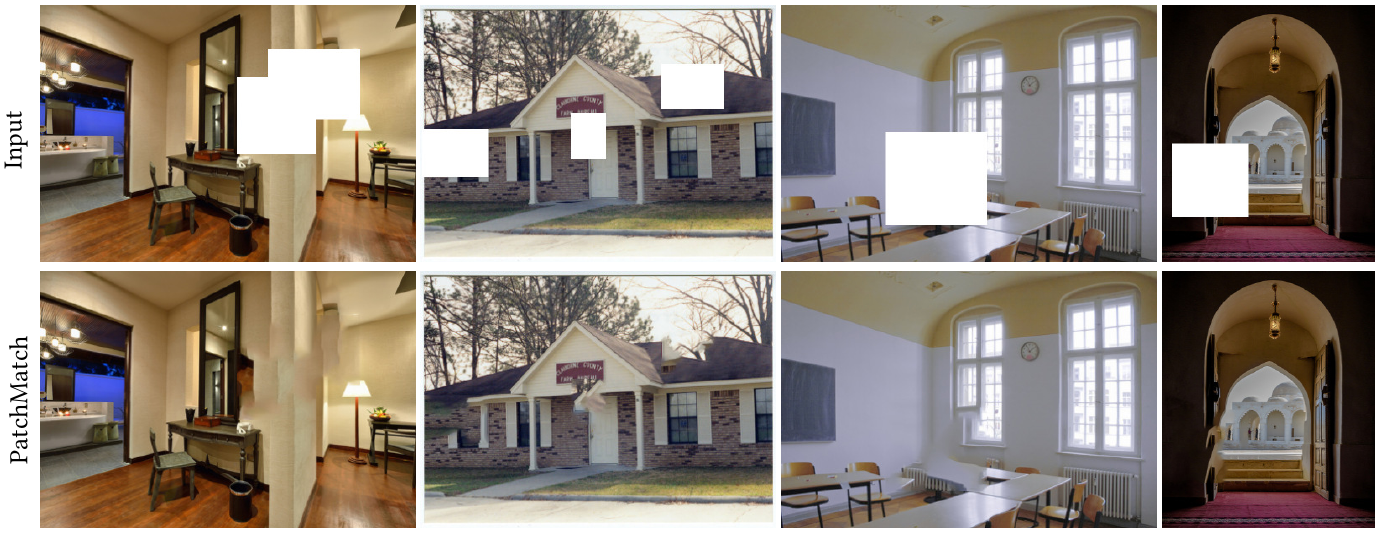
\includegraphics[width=1\linewidth]{IISUKqual1}
	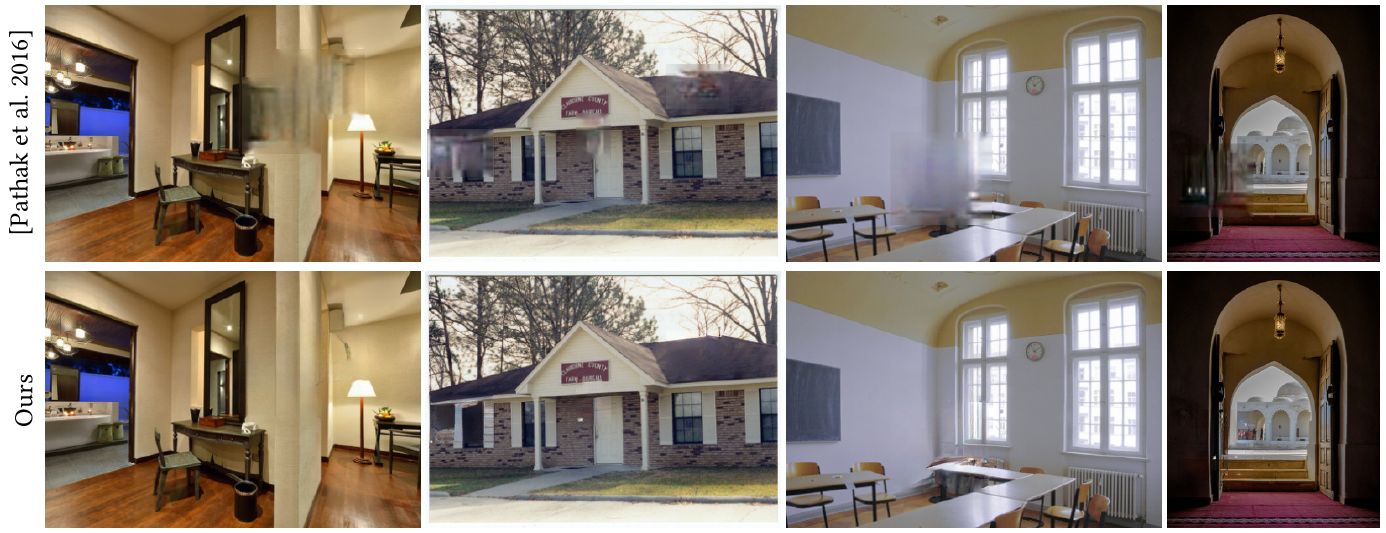
\includegraphics[width=1\linewidth]{IISUKqual2}
	\caption{نتایج کیفی مدل ایزوکا و همکاران در مقایسه با دو روش بیان شده  قبلی بر روی مجموعه‌داده \lr{Places2}}
	\label{fig:iisukqual2}
\end{figure}


\begin{figure}
	\centering
	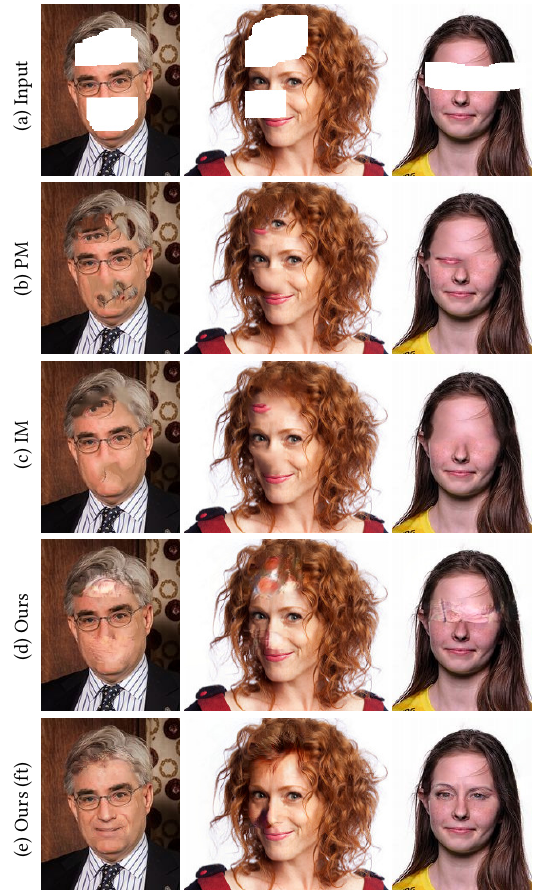
\includegraphics[width=0.5\linewidth]{IISUKqual3}
	\caption{نتایج کیفی مدل ایزوکا و همکاران در مقایسه با دو روش بیان شده  و در مقایسه با معماری ایزوکا، فاین‌تیون شده برای تصاویر چهره. توانایی ساخت ویژگی های نوین چهره در مدل فاین‌تیون شده (FT) مشهود است.}
	\label{fig:iisukqual3}
\end{figure}


\begin{figure}
	\centering
	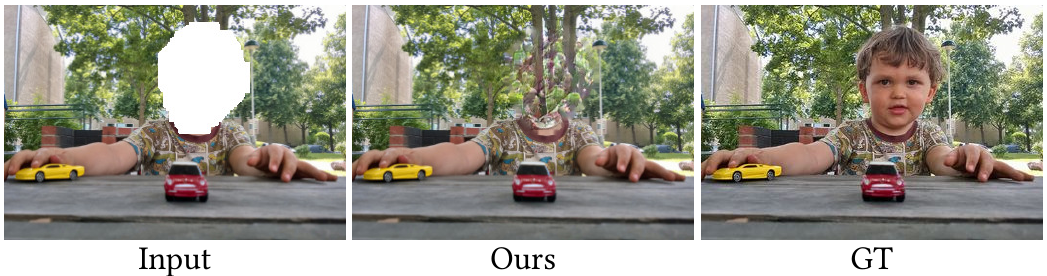
\includegraphics[width=1\linewidth]{IISUKfail}
	\caption{نمونه ای از ترمیم شکست‌خورده توسط معماری ایزوکا و همکاران. مدل آنها نتوانست اشیاء با ساختار بسیار پیچیده را ترمیم کند.}
	\label{fig:iisukfail}
\end{figure}


\warningToSelfExpandable

این استراتژی‌ها همگی به دنبال این هستند که روش‌های مؤثری برای استخراج اطلاعات معتبر از نواحی شناخته‌شده تصویر به منظور پر کردن حفره‌ها پیدا کنند. هدف اصلی این رویکردها، بهره‌برداری بهینه از اطلاعات زمینه‌ای و استفاده از آن‌ها برای بازسازی نواحی گمشده است. با این حال، این روش‌ها هنوز با مشکلی اساسی روبرو هستند: از دست رفتن اطلاعاتی که در فرآیند نمونه‌برداری رو به پایین (\lr{Downsampling}) در شبکه‌های کانولوشنی رخ می‌دهد.  

این فرآیند نمونه‌برداری که برای کاهش ابعاد داده و افزایش بازده محاسباتی در شبکه‌های عصبی مورد استفاده قرار می‌گیرد، اغلب منجر به حذف جزئیات ظریف و اطلاعات ضروری می‌شود که می‌توانند برای بازسازی دقیق‌تر و واقعی‌تر مناطق گمشده نقش کلیدی ایفا کنند. بنابراین، یکی از چالش‌های مهم این است که چگونه می‌توان ضمن بهره‌گیری از مزایای نمونه‌برداری رو به پایین، تأثیرات منفی آن را کاهش داد و اطلاعات از دست رفته را تا حد ممکن حفظ کرد.







\chapter{ترنسفورمر ها و تاریخچه آنها}

از آنجایی که ریشه معماری ترنسفورمر در ترجمه ماشینی و شبکه های عصبی بازگشتی است و معماری های پردازش تصویر بر پایه ترنسفورمر هم به‌شدت از این مفاهیم استفاده می‌کنند، لازم است تا مقدماتی را توضیح دهیم. در این فصل به بررسی RNN ها، شبکه های کاهشی-افزایشی، مکانیزم توجه، معماری ترنسفورمر در حالت خاص ترجمه ماشینی، و در نهایت اقتباس آن‌ها برای عملیات‌های پردازش تصویر می‌پردازیم.

\section{ ترجمه ماشینی}
مسئله ترجمه ماشینی به این صورت تعریف می‌شود که دنباله‌ای از ورودی‌ها $X = \{x_1, x_2, \dots, x_N\}$ در زبان مبدأ داده شده و هدف پیش‌بینی دنباله خروجی $Y = \{y_1, y_2, \dots, y_T\}$ در زبان مقصد است. در اینجا $x_N$ و $ y_T $ به ترتیب به عنوان نشانگر پایان جمله (\texttt{</s>}) در نظر گرفته می‌شوند و $ y_0 $
برابر با شروع جمله (\texttt{<s>}) است. مدل یادگیری ماشین در تلاش برای یافتن عبارت زیر است.

\begin{equation}
\hat{Y} = \arg\max_{Y} P_\theta(Y | X)
\end{equation}

\section{ ترجمه ماشینی بازگشتی}



برای گسترش این فرمول، از قضیه زنجیره‌ای استفاده می‌کنیم تا احتمال شرطی $P_\theta(Y|X)$ را به حاصل‌ضرب احتمالات شرطی تقسیم کنیم:

\begin{align}
	P_{\theta }(Y \mid X) & = P_{\theta }(y_{1:T} \mid X)  \notag \\
	& = P_{\theta }(y_{T} \mid y_{1:T-1}, X) 
	P_{\theta }(y_{T-1} \mid y_{1:T-2}, X)
	...
	P_{\theta }(y_{1} \mid X) \notag \\
	& = \prod_{t=1}^{T} P_\theta(y_t | y_{1:t-1}, X)
\end{align}

فرآیند به این صورت است که مدل، با داشتن ورودی $X$ و دنباله تولید شده تا زمان $t-1$ یعنی $y_{1:t-1}$، احتمال $y_t$ را پیش‌بینی می‌کند. ایده اصلی در مدل‌های ترجمه ماشینی این است که فرایند تولید خروجی $Y$ به صورت ترتیبی انجام می‌شود و در هر مرحله، مدل به خروجی‌های قبلی وابسته است.  برای مدل‌سازی این فرآیند، دو بخش اصلی وجود دارد: کدگذار \lr{(Encoder)} و رمزگشا \lr{(Decoder)}.
\section{شبکه های کدگذار-کدگشا (افزایشی-کاهشی)}
شبکه‌های کدگذار-رمزگشا%
\LTRfootnote{Encoder-Decoder Networks}
یکی از معماری‌های متداول در یادگیری عمیق هستند که به‌طور خاص برای مسائل نیاز1

\subsection{کدگذار (Encoder)}

کدگذار وظیفه دارد اطلاعات توالی ورودی را به یک بازنمایی فشرده تبدیل کند. این فرآیند با استفاده از یک تابع بازگشتی به شکل زیر انجام می‌شود:

$$
h_n = f(x_n, h_{n-1})
$$

که در آن $h_{n-1}$ وضعیت نهان در زمان $ n-1 $ است و $x_n$ ورودی فعلی رمزگذار است.

در نهایت، یک نمایش زمینه‌ای $ c $ با ترکیب بازگشتی بردارهای مخفی $ h $ تولید می‌شود:

$$
c = q(h_{1:N}) = h_N
$$

\subsection{کدگشا (Decoder)}
کدگشا از نمایندگی فشرده تولیدشده توسط کدگذار استفاده کرده و آن را به خروجی مورد نظر نگاشت می‌دهد. این بخش نیز معمولاً از همان نوع شبکه‌های کدگذار استفاده می‌کند، اما با هدف تولید خروجی. فرآیند رمزگشا می‌تواند به شکل مرحله‌به‌مرحله باشد، به‌طوری که هر خروجی تولیدشده به‌عنوان ورودی برای مرحله بعدی استفاده می‌شود.
$$
s_t = g(y_{t-1}, c, s_{t-1})
$$

در اینجا $ g $ تابع تغییر حالت است، $ y_{t-1} $ جاسازی%
\LTRfootnote{Embedding}
آخرین خروجی تخمینی کدگشا است، $s_{t-1}$ آخرین وضعیت نهان کدگشا و $c$ نمایندگی فشرده تولیدشده توسط کدگذار است که یک بازنمایی از کل دنباله ورودی را در بر دارد.

معمولا هر وضعیت نهان $s_t$ به یک عملیات خروجی داده می شود تا در نهایت بدست آید:
$$ P_{\theta}(y_{t} | y_{1:t-1},c) $$

\begin{figure}
	\centering
	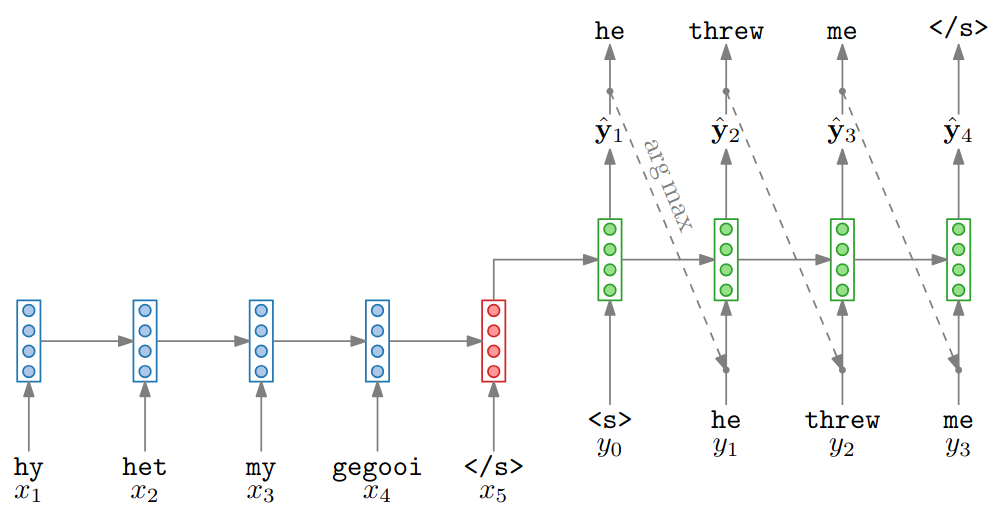
\includegraphics[width=1\linewidth]{figs/rnn_without_attn}
	\caption{نمای کلی یک مدل ترجمه ماشینی بر پایه خروجی های بازگشتی. هدف این شبکه آن است که بازنمایی فشرده و خلاصه ای از کل جمله را در آخرین نشانه ورودی
	($\mathbf{</s>}$)
	جای دهد و کدگشا با تکیه بر همین بردار نهایی، به‌صورت بازگشتی خروجی ترجمه شده را تولید کند.
	}
	\label{fig:rnnwithoutattn}
\end{figure}

در شکل \ref{fig:rnnwithoutattn} یک نمای کلی فرایند های گفته شده در ترجمه کلمه‌به‌کلمه ماشینی بازگشتی ارائه شده است.

یکی از محدودیت‌های اصلی معماری کدگذار-رمزگشا \lr{(Encoder-Decoder) } در مدیریت توالی‌های بلند، وابستگی بیش از حد آن به بردار زمینه \lr{(Context Vector)} است. در این معماری، کدگذار ورودی را به یک بردار فشرده واحد تبدیل می‌کند که حاوی اطلاعات معنایی کل توالی است. سپس رمزگشا از این بردار به‌عنوان منبع اصلی اطلاعات برای تولید خروجی استفاده می‌کند. با افزایش طول توالی ورودی، نمایندگی این بردار فشرده ناکارآمد می‌شود و اطلاعات مهم در فرآیند فشرده‌سازی از بین می‌رود. این محدودیت به‌ویژه در مسائلی مانند ترجمه ماشینی، جایی که وابستگی‌های معنایی میان کلمات دورافتاده وجود دارد، به وضوح دیده می‌شود.

مشکل دیگر این معماری، ناتوانی در حفظ ارتباطات بلندمدت میان بخش‌های توالی است. هنگامی که توالی ورودی شامل اطلاعات متنوع و پیچیده باشد، فشرده‌سازی کل محتوا به یک بردار واحد نمی‌تواند تمامی جزئیات را در خود جای دهد. این امر باعث می‌شود که رمزگشا در بازسازی دقیق اطلاعات ورودی، به‌ویژه برای بخش‌های انتهایی یا نقاطی که با اطلاعات اولیه ورودی وابستگی دارند، دچار ضعف شود. به‌عنوان مثال، در ترجمه یک جمله طولانی، مدل ممکن است ساختار دستوری یا معنای کلمات انتهایی را به دلیل از دست رفتن اطلاعات در بردار زمینه نادیده بگیرد.

همچنین، استفاده از یک بردار ثابت به‌عنوان تنها منبع اطلاعاتی رمزگشا باعث می‌شود که توانایی مدل در مدیریت داده‌های پویا و وابستگی‌های متغیر میان بخش‌های توالی کاهش یابد. این محدودیت‌ها در معماری‌های اولیه مانند \lr{Seq2Seq}، که فاقد مکانیزم توجه بودند، بسیار برجسته بودند. برای حل این مشکل، مکانیزم‌های پیشرفته‌تر مانند مکانیزم توجه و مدل‌های ترنسفورمر معرفی شدند که امکان مدل‌سازی ارتباطات محلی و سراسری را به‌طور همزمان فراهم می‌کنند و وابستگی مدل به یک بردار واحد را از بین می‌برند.

\section{مکانیزم توجه}
مکانیزم توجه%
\LTRfootnote{Attention Mechanism}
\cite{bahdanauNeuralMachineTranslation2016} یک تکنیک پیشرفته در معماری‌های یادگیری عمیق است که به مدل‌ها اجازه می‌دهد به بخش‌های مرتبط‌تر ورودی در هر مرحله از تولید خروجی تمرکز کنند. برخلاف معماری‌های سنتی کدگذار-رمزگشا، که کل اطلاعات ورودی را در یک بردار زمینه فشرده می‌کنند، مکانیزم توجه از ماتریس‌های پرسش 
\lr{(Query)}،
 کلید 
 \lr{(Key)}،
  و مقدار \lr{(Value)}  برای محاسبه وزن‌های توجه استفاده می‌کند. این وزن‌ها نشان‌دهنده میزان اهمیت هر بخش ورودی برای تولید یک بخش خاص از خروجی هستند. با استفاده از عملیات Softmax برای نرمال‌سازی، مدل می‌تواند اطلاعات مربوط به قسمت‌های مهم‌تر ورودی را استخراج کرده و به رمزگشا منتقل کند. این ویژگی باعث می‌شود که مکانیزم توجه بتواند ارتباطات بلندمدت و پیچیده میان بخش‌های مختلف توالی را به‌طور موثر مدل‌سازی کند، که این امر در مسائلی مانند ترجمه ماشینی، خلاصه‌سازی متون، و ترمیم تصاویر بسیار کارآمد است.
  
%  \subsection{مکانیزم خود-توجه\protect\LTRfootnote{Self Attention}}

دنباله ورودی
$$\mathbf{X}_{raw} = [x_1, x_2, \dots, x_N]^T \in \mathbb{R}^{N}$$
را در نظر بگیرید که در آن $N$ طول دنباله است و $ x_i $
\textbf{نشانه}
$i$
ام در این ورودی است. ابتدا هر نشانه باید به یک فضای جاسازی نگاشت شود. مثلا فرض میکنیم که صحبت از پردازش زبان است. هر سمبل ورودی باید به یک «جاسازی کلمه‌ای»%
\LTRfootnote{Word Embedding}
نگاشت شود. مثلا با استفاده از یک «ماتریس واژگان»%
\LTRfootnote{Vocabulary Matrix}.
تابعی که این کار را انجام می‌دهد $ Embedding(symbol) $ می‌نامیم. خواهیم داشت:
 $$
 \mathbf{X}_{\text{embed}} = Embedding(\mathbf{X}_{raw}) \in \mathbb{R}^{N \times D_{embed}}
 $$ 

به طوری که $ D_{embed} $ ابعاد فضای جاسازی است.\\
$ D\_{model} $
را ابعاد فضای نهان مدل در نظر بگیرید که در آن تمام نشانه‌ها و داده‌ها در طول پردازش‌ها و تعاملات مختلف مدل (مانند مکانیزم توجه و لایه‌های تمام متصل) نمایش داده می‌شوند. این بعد معمولاً ابعادی است که برای ذخیره‌سازی و پردازش اطلاعات استفاده می‌شود و در مدل‌های ترنسفورمر معمولاً ثابت است. برای مثال، اگر $ D\_{model}$ برابر ۵۱۲ باشد، تمام توکن‌ها، پس از گذر از لایه‌های ورودی و پردازش‌ها، در فضایی با این ابعاد نمایش داده می‌شوند.

حال نگاشت خطی قابل یادگیری $ \mathbf{E} $ را چنان فرض میکنیم که $ X_{embed} $ را از فضای با ابعاد
$\mathbb{R}^{N \times D_{embed}}$
به فضایی با ابعاد ورودی ترنسفورمر (
$\mathbb{R}^{N \times D\_{model}}$
) ببرد. یعنی
$$
	\mathbf{E} \in \mathbb{R}^{D_{embed} \times D\_{model}}
$$

ورودی $ \mathbf{X} $ را پس از اعمال $\mathbf{E} $ روی $ \mathbf{X}_{\text{embed}} $ و سپس اضافه کردن جاسازی موقعیتی می‌سازیم.

\begin{equation}
	\mathbf{X} = \mathbf{X}_{\text{embed}} + PE \in \mathbb{R}^{N \times D\_{model}}
\end{equation}



ماتریس‌های $\mathbf{Q}$ (پرسش)، $\mathbf{K}$ (کلید) و $\mathbf{V}$ (مقدار) با اعمال نگاشت‌های خطی قابل یادگیری به ماتریس ورودی $\mathbf{X}$ محاسبه می‌شوند:
\begin{align*}
	\mathbf{Q} &= \mathbf{X} \mathbf{W}_Q, \quad \mathbf{W}_Q \in \mathbb{R}^{D \times D_K}, \\
	\mathbf{K} &= \mathbf{X} \mathbf{W}_K, \quad \mathbf{W}_K \in \mathbb{R}^{D \times D_K}, \\
	\mathbf{V} &= \mathbf{X} \mathbf{W}_V, \quad \mathbf{W}_V \in \mathbb{R}^{D \times D_V}.
\end{align*}

در اینجا، $\mathbf{W}_Q$, $\mathbf{W}_K$, و $\mathbf{W}_V$ ماتریس‌های وزن قابل یادگیری هستند.

\textbf{محاسبه امتیاز توجه:} 
امتیاز توجه $\alpha_{i,j}$ نشان‌دهنده میزان اهمیت  نشانه%
\LTRfootnote{Token}
شماره $j$ در ارتباط با نشانه $i$ است. به عبارت دیگر، این امتیاز مشخص می‌کند که نشانه $i$ برای تولید خروجی چقدر باید به اطلاعات نشانه $j$ توجه کند. این فرآیند به مدل اجازه می‌دهد تا وابستگی‌های کوتاه‌برد و بلند‌برد را در دنباله ورودی شناسایی کند. با محاسبه این امتیازات، مدل قادر است مفاهیمی مانند همبستگی معنایی، شباهت متنی و حتی ساختارهای گرامری را استخراج کند، که در بسیاری از مسائل پردازش زبان طبیعی (NLP) اهمیت بالایی دارند. یک امتیاز توجه تعریف شده با تابعی مثل $a$ باید به صورت زیر باشد:

$$
a(q,k_n) \in \mathbb{R}
$$

این امتیاز می‌تواند به روش های مختلفی پیاده‌سازی شود. ساده ترین روش برای محاسبه امتیاز توجه، ضرب نقطه‌ای بردار پرسش و بردار کلید است و  به صورت زیر
$$
a(q,k) = q^{T}k
$$
پیاده‌سازی می‌شود. از معروف‌ترین راه‌های به‌دست آوردن چنین امتیازی، استفاده از «توجه ضرب نقطه ای مقیاس‌یافته»%
\LTRfootnote{Scaled Dot Product Attention}
است:
\begin{align*} 
	a{i,j} &= \frac{\mathbf{q}_i \cdot \mathbf{k}_j}{\sqrt{D_K}},
\end{align*}
که در اینجا $\sqrt{D_K}$ مقیاسی برای جلوگیری از انفجار گرادیان‌ها است.

امتیازات توجه برای تمام نشانه‌ها نرمال‌سازی بیشینه‌نَرم%
\LTRfootnote{Softmax}
شده و سپس ضرب در ماتریس $\mathbf{V}$ می‌شود تا خروجی نهایی تولید شود:


\begin{align}
	\text{Attention}(\mathbf{Q}, \mathbf{K}, \mathbf{V}) = \text{Softmax}\left(\frac{\mathbf{Q} \mathbf{K}^\top}{\sqrt{D_K}}\right) \mathbf{V} \in \mathbb{R}^{N \times D_K}.
\end{align}

در شکل \ref{fig:attncompgraph} گراف محاسباتی بلوک توجه نشان داده شده است.

\begin{figure}
	\centering
	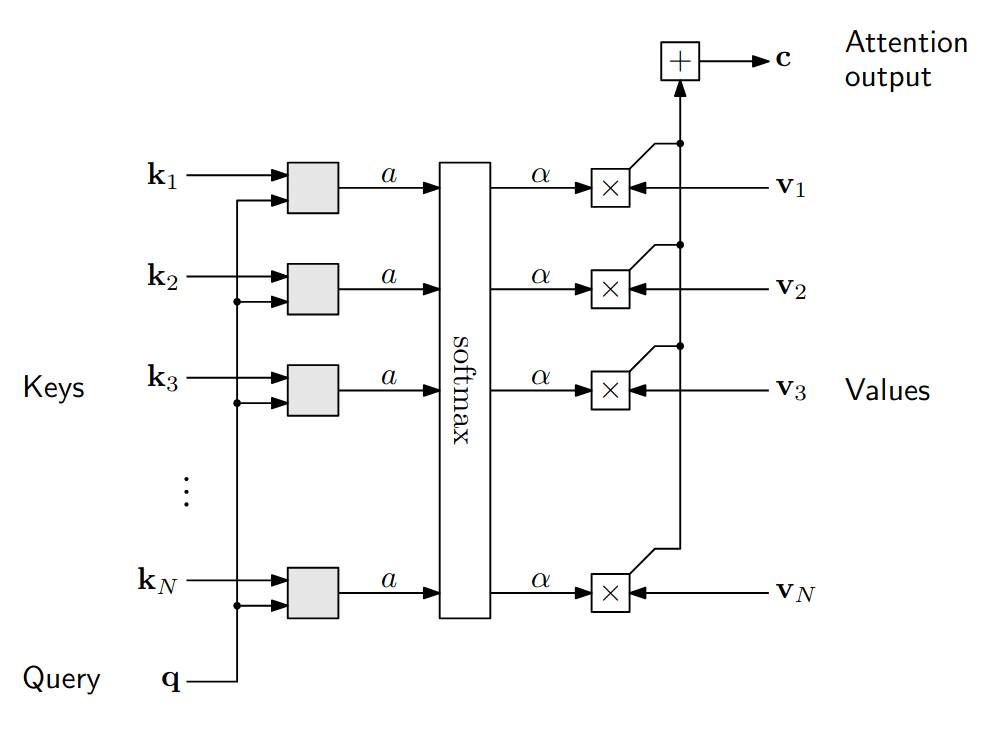
\includegraphics[width=0.7\linewidth]{figs/attnCompGraph}
	\caption{گراف محاسباتی بلوک توجه}
	\label{fig:attncompgraph}
\end{figure}


\textbf{تفسیر امتیاز توجه:}  
یکی از محدودیت‌های مهم در مدل‌های مبتنی بر بردار زمینه‌ای که پیش از ظهور مکانیزم توجه استفاده می‌شد، این بود که تمامی اطلاعات متن به یک بردار واحد فشرده می‌شد. این فشرده‌سازی باعث از دست رفتن بخشی از اطلاعات مهم، خصوصاً در دنباله‌های طولانی، می‌شد. مکانیزم خودتوجه این محدودیت را با تخصیص وزن‌های متفاوت به نشانه‌های مختلف برطرف کرد. به این ترتیب، هر نشانه می‌تواند  بدون نیاز به وابستگی به یک نقطه مرکزی، اطلاعات موردنیاز خود را به‌طور مستقیم از تمامی دیگر نشانه‌ها استخراج کند‍. 

\textbf{تشابه به توجه در زندگی واقعی:}  
مکانیزم توجه شباهت زیادی به نحوه پردازش اطلاعات در ذهن انسان دارد و مستقیما از مدل ذهنی انسان الهام گرفته است. هنگامی که به یک پاراگراف از متن یا یک تصویر نگاه می‌کنیم، توجه ما به بخش‌های مختلف بسته به اهمیت آنها جلب می‌شود. برای مثال، هنگام خواندن یک جمله، ممکن است بر کلمات کلیدی تمرکز کنیم که برای درک معنای کلی ضروری هستند. مکانیزم توجه در شبکه‌های عصبی نیز به‌طور مشابه عمل می‌کند و وزن بیشتری به اطلاعات مرتبط‌تر اختصاص می‌دهد، در حالی که اطلاعات کم‌اهمیت‌تر را نادیده می‌گیرد. این فرآیند باعث بهبود کارایی مدل ها می‌شود؛ چرا که به مدل توانایی دسترسی با وزن دلخواه به هر بخشی از ورودی را می‌دهد.

\section{مکانیزم خودتوجه در معماری های کاهشی-افزایشی}
اگرچه مکانیزم خودتوجه اغلب به‌عنوان یکی از ویژگی‌های برجسته معماری‌های ترنسفورمر شناخته می‌شود، می‌توان آن را به معماری‌های بازگشتی نیز اضافه کرد تا محدودیت‌های آن‌ها در مدیریت وابستگی‌های بلندمدت کاهش یابد. ایده این است که به جای وابستگی صرف به حالات بازگشتی، رمزگذار و رمزگشا می‌توانند با استفاده از مکانیزم خود-توجه، ارتباطات مستقیم بین نشانه‌های ورودی یا خروجی را مدلسازی کنند.

در هنگام رمزگشایی‌، بجای استفاده از بردار واحد $c$ که می‌توانست موجب از دست رفتن اطلاعات شود،‌ برای هر گام زمانی $t$ یک بردار زمینه $c_t$ محاسبه می‌کنیم. این محاسبه بر پایه مکانیزم خودتوجه است؛ به این صورت که Value ها و Key ها همان وضعیت های نهان  \textbf{کدگذار} (${h_1, h_2, \dots, h_N}$ ) و Query مقدار فعلی حالت پنهان \textbf{کدگشا} است.

کلیدها ($\mathbf{K}$): نمایانگر ویژگی‌های رمزگذاری‌شده توالی ورودی هستند که از حالات پنهان انکدر استخراج می‌شوند: 
$$
K = \{h_1, h_2, \dots, h_N\},
$$
که در آن $ h_n $​ حالت پنهان کدگشا در گام زمانی $\mathbf{n}$ است.

مقادیر ($\mathbf{V}$): شامل همان اطلاعات کلید ها هستند. در اصل مقادیر بردار هایی هستند که امتیاز $\alpha$ توجه بر آن ها اعمال شده و میانگین وزنی مقادیر است که بردار $c_t$ را می‌سازد.
$$
K = \{h_1, h_2, \dots, h_N\},
$$
که در آن $ h_n $​ حالت پنهان کدگشا در گام زمانی $\mathbf{n}$ است.


پرسش‌ها ($\mathbf{Q}$):
نمایانگر حالت پنهان فعلی دیکدر در گام زمانی  $t-1 $ هستند:  
$$
Q = s_{t-1},
$$
که در آن \( s_{t-1} \) حالت پنهان دیکدر در گام زمانی قبلی است.

امتیاز هم‌راستایی بین کوئری $Q$ و هر کلید $ K_n $  با استفاده از تابع امتیازدهی محاسبه می شود که قبلا توضیح داده شد.
$$
a_{t, n} = \text{score}(Q, K_n).
$$

سپس این امتیاز ها بیشینه‌نرم شده و وزن های توجه را می‌سازند.
$$
\alpha_{t, n} = \frac{\exp(a_{t, n})}{\sum_{n'=1}^N \exp(a_{t, n'})}.
$$

بردار زمینه  
بردار زمینه $ c_t $ در گام تولید $t$ به صورت ترکیب وزنی مقادیر $\mathbf{V}$
محاسبه می‌شود:  
$$
c_t = \sum_{n=1}^N \alpha_{t, n} h_n.
$$


 کدگشا مانند قبل بروزرسانی می‌شود.  
$$
s_t = g(y_{t-1}, c_t, s_{t-1}),
$$
که در آن $g$ معمولاً یک \lr{RNN}، یک
LSTM
 یا GRU است.

این مکانیزم به‌صورت پویا تعیین می‌کند که کدام توکن‌های ورودی برای گام فعلی دیکدر مهم‌تر هستند. این ویژگی نه تنها عملکرد بهتری بر روی توالی‌های بلند ارائه می‌دهد، بلکه با نمایش وزن‌های توجه $\alpha_{t,n}$ امکان تفسیر مدل را هم فراهم می‌کند و وابستگی مدل به یک بردار واحد را کم می‌کند. به وضوح این روش نیازمند محاسبات بیشتری است و از پیچیدگی زمانی بیشتری برخوردار است.

\section{مدل‌های ترنسفورمر}

مدل‌های ترنسفورمر که برای اولین بار در \cite{vaswaniAttentionAllYou2023} معرفی شدند، به‌طور کلی از معماری‌های جدیدی بهره می‌برند که از مکانیزم توجه به‌طور کامل استفاده می‌کنند. برخلاف مدل‌های سنتی seq2seq که از RNN یا LSTM برای پردازش توالی‌ها استفاده می‌کنند، ترنسفورمرها نیازی به پردازش ترتیبی ورودی‌ها ندارند و می‌توانند به‌طور همزمان کل توالی ورودی را پردازش کنند. این امر موجب می‌شود که مدل‌های ترنسفورمر برای پردازش داده‌های توالی بلند بسیار کارآمدتر از مدل‌های مبتنی بر RNN یا LSTM باشند.

در این بخش، به بررسی معماری ترنسفورمر و اجزای آن می‌پردازیم، از جمله مکانیزم توجه چندگانه، و معرفی مکانیزمی به نام جاسازی موقعیتی%
\LTRfootnote{Positional Embedding}
برای پردازش توالی‌های ورودی در مدلی که هدف آن موازی سازی است.
\subsection{مکانیزم توجه چندگانه}
در مدل‌های ترنسفورمر، توجه چندگانه به این صورت عمل می‌کند که چندین «سر توجه»%
\LTRfootnote{Attention Head}
به طور موازی اجرا می‌شوند و توزیع های توجه مختلفی محاسبه می‌کنند. به طوری که هر «سر» توجه، امتیاز و وزن های توجه مستقل خودش را محاسبه می‌کند و به ابعاد خاصی از ورودی نگاه می‌کند. این امر به مدل این امکان را می‌دهد که روابط وسیع و گسترده تر و دقیق تری را کشف کند. در نهایت نتیجه همه «سر» ها تجمیع شده و به یک بازنمایی نهایی تبدیل می‌شوند.

ابتدا ورودی به چندین «سر» مختلف تقسیم می‌شود. برای این منظور، بردارهای پرس و جو (\lr{Query})، کلید (\lr{Key})، و مقدار (\lr{Value}) با استفاده از تبدیلات خطیِ مستقل به زیرفضاهای کم‌بُعدتر (\lr{Subspaces}) تصویر می‌شوند. هر سر توجه، این بردارهای تبدیل‌شده را دریافت کرده و با مکانیزم توجه نقطه‌ای-ضربی مقیاس‌شده (\lr{Scaled Dot-Product Attention}) پردازش می‌کند. در این فرآیند، هر سر به بخش‌های متفاوتی از فضای نمایشی ورودی تمرکز می‌کند و الگوهای معنایی یا نحوی خاصی را استخراج می‌نماید.

پس از محاسبه خروجی هر سر، تمامی نتایج به یک بردار واحد الحاق (\lr{Concatenate}) شده و مجدداً از طریق یک تبدیل خطی دیگر به ابعاد مطلوب بازتابانده می‌شوند. این رویکرد دو مزیت عمده دارد: اولاً امکان یادگیری روابط پیچیدهتر با ترکیب اطلاعات از زوایای مختلف فضای نمایشی، و ثانیاً افزایش ظرفیت مدل بدون ایجاد وابستگی بیش از حد به هر یک از سرهای توجه. به این ترتیب، مدل می‌تواند همزمان به انواع متفاوتی از وابستگی‌های بین توکن‌ها (مثلاً روابط دستوری، معنایی یا موقعیتی) توجه کند که این امر قدرت تعمیم‌پذیری ترنسفورمرها را به شدت افزایش می‌دهد. هر «سر توجه» صاحب نگاشت های خطی قابل یادگیری مخصوص خود است.

فرض کنید ورودی (پیش‌پردازش شده) اصلی، ماتریس 
$\mathbf{X} \in \mathbb{R}^{N \times D\_{model}}$
باشد که 
$N$ تعداد توکن‌ها و 
$D_{\text{model}}$ 
بُعد نهفتگی است. برای ایجاد $h$ سر توجه بعد نهفتگی هر «سر» را مشخص کنیم.
$$
D\_{head} = D\_{model} / h
$$
برای هر سر \(i\) (که \(i = 1, \dots, h\))، ماتریس‌های وزن قابل یادگیری زیر را تعریف می‌کنیم:  
\begin{align*}
	\mathbf{W}_i^Q &\in \mathbb{R}^{D\_{model} \times D\_{head}} \quad \text{(نگاشت خطی پرس‌وجو)}, \\
	\mathbf{W}_i^K &\in \mathbb{R}^{D\_{model} \times D\_{head}} \quad \text{(نگاشت خطی کلید)}, \\
	\mathbf{W}_i^V &\in \mathbb{R}^{D\_{model} \times D\_{head}} \quad \text{(نگاشت خطی مقدار)}.
\end{align*}

برای سر \(i\)، ورودی \(\mathbf{X}\) را به پرس‌وجو، کلید و مقدار تبدیل می‌کنیم:  
\begin{align*}
	\mathbf{Q}_i &= \mathbf{X} \mathbf{W}_i^Q \in \mathbb{R}^{N \times D\_{head}}, \\
	\mathbf{K}_i &= \mathbf{X} \mathbf{W}_i^K \in \mathbb{R}^{N \times D\_{head}}, \\
	\mathbf{V}_i &= \mathbf{X} \mathbf{W}_i^V \in \mathbb{R}^{N \times D\_{head}}.
\end{align*}

برای سر \(i\)، امتیازهای توجه و خروجی را محاسبه می‌کنیم:  
$$
\text{head}_i = \text{Attention}(\mathbf{Q}_i, \mathbf{K}_i, \mathbf{V}_i) = \text{softmax}\left(\frac{\mathbf{Q}_i \mathbf{K}_i^T}{\sqrt{D\_{head}}}\right) \mathbf{V}_i \in \mathbb{R}^{N \times D\_{head}}.
$$

در نهایت خروجی همه «سر» ها الحاق می‌شوند، یک نگاشت خطی قابل یاگیری
$\mathbf{W}^O$
اعمال می‌کنیم و داریم:
$$
\text{MultiHead}(\mathbf{X}) = \text{Concat}(\text{head}_1, \dots, \text{head}_H) \mathbf{W}^O \in \mathbb{R}^{N \times D\_{model}},
$$
به طوری که
%$$
%\text{head}_i = \text{Attention}(QW_i^Q, KW_i^K, VW_i^V).
%$$
%و
$$
\mathbf{W}^O \in \mathbb{R}^{h \cdot D_{\text{head}} \times D_{\text{model}}}.
$$

در شکل \ref{fig:mhattn1} گرافی برای این عملیات ارائه شده است.

\subsection{جاسازی موقعیتی}

مدل‌های ترنسفورمر به طور ذاتی ترتیبی نیستند. این ویژگی یکی از عوامل اصلی موفقیت آنها محسوب می‌شود. در مقابل، مدل‌های بازگشتی مثل Seq2Seq به طور ذاتی ترتیبی هستند. این بدان معناست که پردازش ورودی‌ها در این مدل‌ها به صورت گام به گام انجام می‌شود و اطلاعات ورودی به صورت ترتیبی وارد مدل می‌شود. سؤال اصلی این است که چگونه می‌توان از این ویژگی ترتیبی مدل‌های RNN برای وظایف پردازش زبان استفاده کرد، هنگامی که معماری ما به یک معماری غیرترتیبی مثل ترنسفومر تغییر می‌یابد؟

تحقیقات نشان داد که می‌توان با استفاده از جاسازی موقعیتی، این مشکل را حل کرد. در این روش، برای مدل ترنسفورمر که به طور ذاتی ترتیبی نیست، اطلاعات موقعیتی به ورودی‌ها اضافه می‌شود. این امر به مدل این امکان را می‌دهد که ترتیب و موقعیت هر نشانه در توالی را در نظر بگیرد، بدون اینکه نیاز به پردازش ترتیبی ورودی‌ها باشد. به عبارت دیگر، \textbf{مدل‌های ترنسفورمر می‌توانند از طریق این جاسازی موقعیتی به صورت غیر ترتیبی عمل کنند، و در عین حال همچنان ویژگی‌های ترتیبی توالی‌ها را درک کنند}.

در این روش، به هر توکن ورودی یک بردار موقعیتی اضافه می‌شود تا اطلاعات مربوط به ترتیب آن در توالی به مدل منتقل شود. این بردارهای موقعیتی می‌توانند به‌طور دلخواه تولید شوند یا حتی میتوانند مانند نگاشت‌های خطی جاسازی، ماتریس هایی قابل‌آموزش باشند. Vaswani و همکاران در تحقیق خود چنین برداری را  به صورت زیر تعریف کرده اند:

\begin{equation}
PE(t, 2i) = \sin\left( \frac{t}{\lambda^{2i/d}} \right), \quad PE(t, 2i+1) = \cos\left( \frac{t}{\lambda^{2i/d}} \right)
\end{equation}
که در آن:
$t$ شماره توکن در توالی است،
$i$ شاخص بعد در بردار موقعیتی است،
و
$d$ ابعاد کل بردار موقعیتی است. 
همچنین $\lambda$ پیشنهاد شده توسط Vaswani و همکاران عدد ۱۰۰۰۰ (ده هزار) است که بسته به طول زمینه%
\LTRfootnote{Context Length}
مورد نظر در دنباله های ورودی، می‌تواند متغیر باشد. این بردارهای موقعیتی به ورودی‌ها اضافه می‌شوند و به مدل این امکان را می‌دهند که ترتیب نشانه‌ها را در توالی در نظر بگیرد.

\begin{figure}
	\centering
	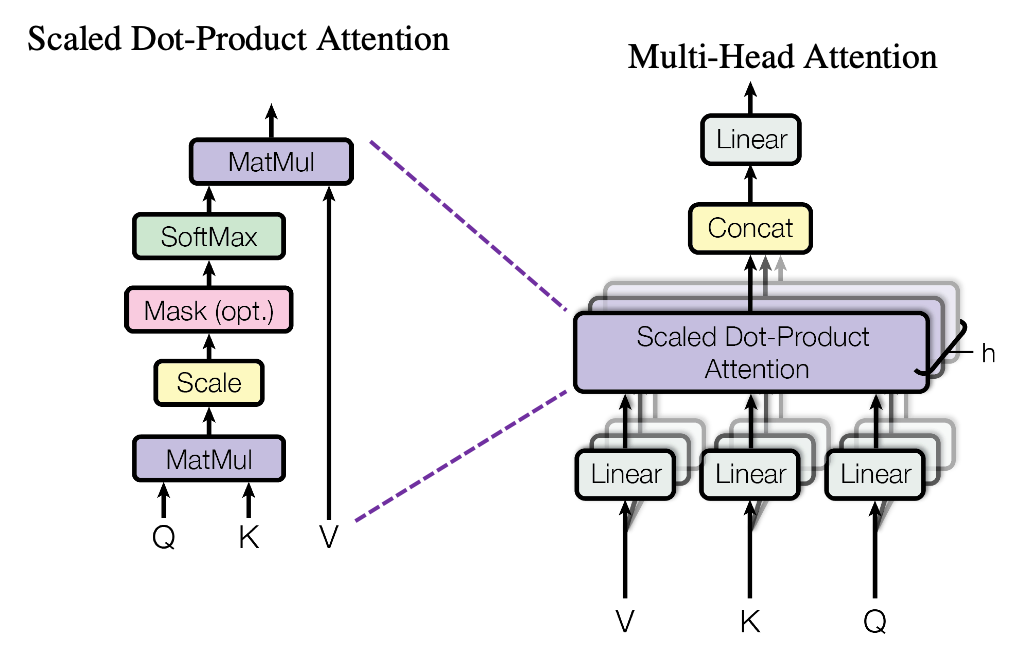
\includegraphics[width=0.7\linewidth]{figs/mhattn1.png}
	\caption{دیاگرام معماری توجه چندگانه. ماتریس $Q$ ماتریس پرسش، ماتریس $K$ ماتریس کلید و ماتریس $V$ مقدار اختصاص یافته به آن کلید است. در هر «سر» توجه همانند قبل از توجه ضرب‌نقطه‌ای استفاده می‌شود.}
	\label{fig:mhattn1}
\end{figure}

%
%\subsection*{ساختار مدل ترنسفورمر}
%مدل ترنسفورمر از دو بخش اصلی تشکیل شده است: رمزگذار و رمزگشا. هر یک از این بخش‌ها شامل چندین لایه هستند که هر کدام شامل مکانیزم‌های توجه چندگانه و یک شبکه عصبی کاملاً متصل (Feed-Forward Neural Network) هستند. در هر لایه، ابتدا توجه چندگانه اعمال می‌شود، سپس نتیجه با یک شبکه عصبی کاملاً متصل (FCN) پردازش می‌شود و در نهایت با استفاده از یک نرمال‌سازی و اعمال یک لایه کانولوشنی، نتیجه نهایی به‌دست می‌آید.


%
%\subsection*{معادلات ترنسفورمر}
%مدل ترنسفورمر به طور خلاصه شامل مراحل زیر است:
%
%1. **لایه توجه چندگانه**:
%\[
%\text{MultiHead}(Q, K, V) = \text{Concat}(\text{head}_1, \dots, \text{head}_h) W^O
%\]
%که هر سر توجه به صورت زیر عمل می‌کند:
%\[
%\text{head}_i = \text{Attention}(Q W_i^Q, K W_i^K, V W_i^V)
%\]
%
%2. **شبکه عصبی کاملاً متصل**:
%\[
%\text{FFN}(x) = \max(0, x W_1 + b_1) W_2 + b_2
%\]
%که در آن \( W_1 \)، \( W_2 \) ماتریس‌های وزن و \( b_1 \)، \( b_2 \) بایاس‌ها هستند.
%
%3. **ساختار انکدر**:
%هر لایه انکدر شامل یک لایه توجه چندگانه و یک شبکه عصبی کاملاً متصل است:
%\[
%\text{EncoderLayer}(x) = \text{FFN}(\text{MultiHeadAttention}(x))
%\]
%این لایه‌ها به‌طور متوالی برای پردازش ورودی‌ها تکرار می‌شوند.
%
%4. **ساختار دیکدر**:
%دیکدر نیز مشابه انکدر است، اما تفاوت اصلی آن این است که ابتدا از توجه ماسک‌شده برای جلوگیری از دسترسی به آینده استفاده می‌کند. معادله مربوط به دیکدر به صورت زیر است:
%\[
%\text{DecoderLayer}(x) = \text{FFN}(\text{MultiHeadAttention}(\text{Masked}(x), \text{EncoderOutput}))
%\]
%در اینجا \( \text{Masked}(x) \) به این معنا است که توجه به ورودی‌ها تنها به توکن‌های قبلی محدود می‌شود.


\section{ترنسفورمر ها در ترمیم تصویر}

خاصیت های مطرح شده و موفقیت شگرف مدل های ترنسفورمر
\cite{radfordLanguageModelsAre2019}
\cite{brownLanguageModelsAre2020}
\cite{openaiGPT4TechnicalReport2024}
در مدل سازی دنباله های متنی طولانی، بدون از دست رفتن وابستگی های بلندمدت، موجب جلب توجه محققان به کاربرد آن‌ها در کابرد های پردازش تصویر نیز شده است.
\cite{liuSwinTransformerHierarchical2021}


یکی از اولین مدل‌های مطرح در این زمینه، مدل ویت (ViT) 
\cite{dosovitskiyImageWorth16x162021}
است که تصویر ورودی را به قطعات کوچک (پچ‌ها) تقسیم کرده و از این قطعه‌ها به عنوان دنباله ورودی به مدل استفاده می‌کند. اما این مدل صرفا یک مدل طبقه بندی است. در فصل بعد روش پیشنهادی ای ارائه می‌دهیم که با الهام گیری از قطعه‌بندی تصویر، یک مدل ترمیم تصویر بر پایه ترنسفورمر بسازیم. 






%
\chapter{آزمایشات و نتایج جدید}

در این فصل ما آزمایشات خود را مبنی بر پیاده سازی مدل هایی مبتنی بر معماری xLSTM برای ترمیم تصاویر ایستا بررسی و تفسیر می‌کنیم. مشاهداتی بر مدل سازی داده های غیرزمانی توسط معماری های زمانی مانند LSTM ارائه کرده و علل مد نظر خود را شرح و توجیه می‌کنیم.

\section{استفاده از LSTM و xLSTM در ترمیم تصویر}

در حالی که روش‌های سنتی و رویکردهای مدرن یادگیری عمیق مانند شبکه‌های عصبی پیچشی (CNN) و ترنسفورمرها موفقیت قابل توجهی نشان داده‌اند، شبکه‌های عصبی بازگشتی (RNN)، به‌ویژه شبکه‌های حافظه بلندمدت کوتاه‌مدت (LSTM)، برای این وظیفه کمتر مورد بررسی قرار گرفته‌اند. این کار به بررسی کاربرد معماری نوآورانه xLSTM در تکمیل تصویر یک‌تایی می‌پردازد و تمرکز آن بر روی جنبه‌های خروجی مدل است. ما به بررسی مبانی ریاضی، رفتار معماری و چالش‌هایی که در طول آزمایش‌ها با آن‌ها مواجه شدیم خواهیم پرداخت.

\subsection{معرفی مختصر LSTM}
شبکه‌های حافظه طولانی-کوتاه‌مدت (\lr{Long Short-Term Memory} یا \lr{LSTM})
\cite{hochreiterLongShortTermMemory1997}
، یک نوع خاص از شبکه‌های عصبی بازگشتی هستند که برای یادگیری وابستگی‌های بلندمدت در داده‌های دنباله‌ای طراحی شده‌اند. LSTM ها با استفاده از سلول‌های حافظه و مکانیزم‌های دروازه‌ای، مشکل فراموشی گرادیان که در شبکه‌های RNN سنتی رخ می‌دهد را کاهش می‌دهند. 

شبکه‌های عصبی بازگشتی بلند-کوتاه‌مدت (LSTM) از نظر ساختاری شباهت‌هایی به شبکه‌های عصبی بازگشتی استاندارد دارند، اما با این تفاوت که در اینجا هر گره بازگشتی معمولی با یک سلول حافظه جایگزین شده است. هر سلول حافظه شامل یک حالت داخلی است که به عنوان یک گره با اتصال بازگشتی خودکار و وزن ثابت 1 عمل می‌کند. این ویژگی منحصر به فرد باعث می‌شود که گرادیان‌ها بتوانند در طول گام‌های زمانی متعدد بدون مواجهه با مشکلاتی مانند ناپدید شدن (Vanishing) یا انفجار (Exploding) گرادیان، منتقل شوند. این مکانیسم به شبکه‌های LSTM امکان می‌دهد تا وابستگی‌های بلندمدت را در داده‌های متوالی به طور مؤثرتری یاد بگیرند و حفظ کنند.

\begin{figure}
	\centering
	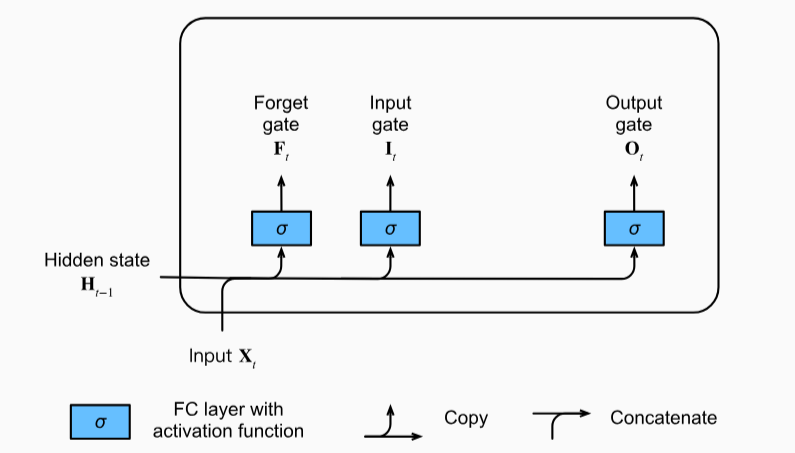
\includegraphics[width=0.7\linewidth]{lstm1}
	\caption{محاسبه گیت ورودی،‌ فراموشی و خروجی در یک سلول LSTM}
	\label{fig:lstm1}
\end{figure}

در مدل‌های شبکه‌های عصبی بازگشتی (RNN)، فرض کنید که تعداد واحدهای پنهان برابر با \( h \)، اندازه دسته برابر با \( n \) و تعداد ورودی‌ها برابر با \( d \) باشد. بنابراین، ورودی به شبکه در زمان گام \( t \) به صورت \( \mathbf{X}_t \in \mathbb{R}^{n \times d} \) و وضعیت پنهان گام زمانی قبلی به صورت \( \mathbf{H}_{t-1} \in \mathbb{R}^{n \times h} \) تعریف می‌شود. به طور مشابه، در هر زمان گام \( t \)، گیت‌ها به شرح زیر تعریف می‌شوند: گیت ورودی \( \mathbf{I}_t \in \mathbb{R}^{n \times h} \)، گیت فراموشی \( \mathbf{F}_t \in \mathbb{R}^{n \times h} \) و گیت خروجی \( \mathbf{O}_t \in \mathbb{R}^{n \times h} \). این گیت‌ها به صورت زیر محاسبه می‌شوند:

\[
\begin{aligned}
	\mathbf{I}_t &= \sigma(\mathbf{X}_t \mathbf{W}_{\textrm{xi}} + \mathbf{H}_{t-1} \mathbf{W}_{\textrm{hi}} + \mathbf{b}_\textrm{i}),\\
	\mathbf{F}_t &= \sigma(\mathbf{X}_t \mathbf{W}_{\textrm{xf}} + \mathbf{H}_{t-1} \mathbf{W}_{\textrm{hf}} + \mathbf{b}_\textrm{f}),\\
	\mathbf{O}_t &= \sigma(\mathbf{X}_t \mathbf{W}_{\textrm{xo}} + \mathbf{H}_{t-1} \mathbf{W}_{\textrm{ho}} + \mathbf{b}_\textrm{o}),
\end{aligned}
\]

که در آن \( \mathbf{W}_{\textrm{xi}}, \mathbf{W}_{\textrm{xf}}, \mathbf{W}_{\textrm{xo}} \in \mathbb{R}^{d \times h} \) و \( \mathbf{W}_{\textrm{hi}}, \mathbf{W}_{\textrm{hf}}, \mathbf{W}_{\textrm{ho}} \in \mathbb{R}^{h \times h} \) پارامترهای وزن هستند و \( \mathbf{b}_\textrm{i}, \mathbf{b}_\textrm{f}, \mathbf{b}_\textrm{o} \in \mathbb{R}^{1 \times h} \) پارامترهای بایاس هستند. در اینجا، از توابع سیگموید استفاده می‌شود تا مقادیر ورودی به بازه \( (0, 1) \) نگاشت شوند.


\subsection{جمع‌بندی}
اگرچه استفاده از LSTM و xLSTM برای ترمیم تصاویر به‌عنوان یک رویکرد نوآورانه مطرح شد، اما عدم وجود روابط زمانی در داده‌های تصویری و محدودیت‌های معماری شبکه‌های بازگشتی، کارایی این روش‌ها را محدود کرد. در نهایت، این مشاهدات نشان داد که ترکیب معماری‌های مبتنی بر توجه با سایر مکانیزم‌های بازنمایی مکانی، مانند Grid Embeddings، برای حل این مسئله ضروری است.


%
\فصل{نتیجه‌گیری}

در این فصل، ضمن جمع‌بندی نتایج جدید ارائه‌شده در پایان‌نامه یا رساله، 
مسائل باز باقی‌مانده و همچنین پیشنهادهایی برای ادامه‌ی کار ارائه می‌شوند.



% -------------- Bibliography & Dictionary ---------------


% -------------------------------------------------------
%  Bibliography
% -------------------------------------------------------

\clearpage
\phantomsection
\renewcommand\bibname{\flushright{\rl{مراجع}}}
\addcontentsline{toc}{chapter}{مراجع}

\begin{latin}
    \baselineskip=.8\baselineskip
    \bibliographystyle{./styles/packages/unsrtabbrv}

    % Uncomment next line to include uncited references
    % \nocite{*}

    \bibliography{bibs/full,bibs/refs}
\end{latin}

\clearpage
\phantomsection
\addcontentsline{toc}{chapter}{واژه‌نامه}

\chapter*{واژه‌نامه}
\begin{multicols}{2}
\small

\dicalphabet{الف}
\dic{Heuristic}{ابتکاری}


\dicalphabet{ب}


\dicalphabet{پ}
\dic{Complexity}{پیچیدگی}

\dicalphabet{ت}
\dic{Emperical}{تجربی}
\dic{Distributed}{توزیع‌شده}

\dicalphabet{ج}
\dic{separable}{جداپذیر}


\dicalphabet{ح}

\dicalphabet{خ}
\dic{Auto-Encoder}{خودرمزگذار}
\dic{Self Attention}{مکانیزم خودتوجه}

\dicalphabet{د}
\dic{Data}{داده}


\dicalphabet{ر}


\dicalphabet{ز}


\dicalphabet{س}
\dic{Hierarchichal}{سلسه‌مراتبی}

\dicalphabet{ش}
\dic{Pseudocode}{شبه کد}
\dic{Object}{شیء}

\dicalphabet{ص}


\dicalphabet{غ}

\dicalphabet{ف}


\dicalphabet{ق}
\dic{Deterministic}{قابل پیش‌بینی}

\dicalphabet{ک}
\dic{Efficient}{کارا}
\dic{Encoder-Decoder}{کدگذار-رمزگشا}


\dicalphabet{گ}
%\dic{pass}{گذر}

\dicalphabet{م}
\dic{Parallelization}{موازی‌سازی}


\dicalphabet{ن}
\dic{Token}{نشانه}
\dic{Projection}{نگاشت}

\dicalphabet{هـ}


\dicalphabet{ی}


\end{multicols}




% -------------------- Appendices --------------------

%\begin{appendix}
%    \include{chapters/appendix}
%\end{appendix}


% -------------------- English Pages --------------------

%\newgeometry{left=3cm,right=2.5cm}

%\pagestyle{empty}
%
% -------------------------------------------------------
%  English Abstract
% -------------------------------------------------------

\begin{latin}

\begin{center}
\textbf{Abstract}
\end{center}
\baselineskip=.8\baselineskip

We present a standard template for typesetting theses in Persian. 
The template is based on the \XePersian\ package for the \LaTeX\ typesetting system.
This write-up shows a sample usage of this template.


\bigskip\noindent\textbf{Keywords}:
Thesis, Typesetting, Template, \XePersian\

\end{latin}

%
% -------------------------------------------------------
%  English Title Page
% -------------------------------------------------------

\begin{center}

\begin{latin}


\includegraphics[scale=0.25]{front/template/images/logo}

\EnglishThesisUniversity \\
\EnglishThesisDepartment

\begin{large}
\vspace{0.7cm}
\EnglishThesisDegree{} Thesis


\vspace{1.5cm}

{\Large\textbf\EnglishThesisTitle}

\vspace{1.5cm}

{\normalsize By:}\\
\textbf{\EnglishThesisAuthor}

\vspace{1cm}

{\normalsize Supervisor:}\\ 
\textbf{\EnglishThesisSupervisor}

\end{large}

\vspace{1.5cm}
\EnglishThesisDate

\end{latin}

\end{center}



% -------------------- The End! --------------------

\end{document}

